\documentclass[pre,twocolumn,superscriptaddress,longbibliography,nofootinbib,floatfix]{revtex4-2}

\usepackage{amsmath,amssymb,amsthm}
\usepackage{graphicx}
\usepackage{booktabs}
\usepackage{bm}
\usepackage{placeins}
\usepackage{xr-hyper}
\usepackage[colorlinks=true,citecolor=blue,linkcolor=blue,urlcolor=blue]{hyperref}

\newtheorem{theorem}{Theorem}
\newtheorem{proposition}{Proposition}
\newtheorem{lemma}{Lemma}
\newtheorem{corollary}{Corollary}

% labels of the Supplemental Material (Tables S1-..., Figs. S1-...); compile supp.tex too
\externaldocument{supp}

\begin{document}

\title{Overlapping communities as connected components of a commonality hypergraph}

% Author order confirmed: Deinega, Kanovsky, Barzel (as in the M.Sc. thesis with Barzel in place of Levit).
% TODO(Dima): Kanovsky's department at Yezreel Valley College.
\author{Dmitri Deinega}
\affiliation{Department of Mathematics, Bar-Ilan University, Ramat Gan 5290002, Israel}
\author{Igor Kanovsky}
\affiliation{Max Stern Yezreel Valley College, Emek Yezreel, Israel}
\author{Baruch Barzel}
\affiliation{Department of Mathematics, Bar-Ilan University, Ramat Gan 5290002, Israel}

\begin{abstract}
Nodes that share most of their neighbours tend to share a community. On this premise,
three nodes, one adjacent to the other two, whose three pairs all reach a commonality
threshold form an elementary community, and communities are the connected components of
the resulting 3-uniform hypergraph under shared pairs. The construction, HyperCommon, is
deterministic, local and nested in its threshold, and no pair of nodes binds two
communities. Its cost is linear in the number of wedges, which an exact pruning of hub
wedges keeps below $12\,m\ln m$ on thirty-two real networks with $m$ edges. We derive the
exact window of thresholds that recovers planted overlapping ring lattices. Compared with
fourteen other methods, every parameter chosen without labels, HyperCommon is the most
accurate in fifteen of twenty-eight ring-lattice settings and level in six, most clearly
where communities of unequal size and density overlap. It trails on all eight families
of overlapping LFR graphs, and on the rings once a tenth (with labels) or three tenths
(without) of their edges are rewired internally: it needs communities whose members share
many neighbours. On seventeen real networks of up to $1.1\times10^6$ nodes, the threshold
chosen without labels keeps a median 94\% of the best threshold's F1, but on most of
them another method is more accurate.

\end{abstract}

\maketitle

% ---------------------------------------------------------------------------
\section{Introduction}
\label{sec:intro}
% ---------------------------------------------------------------------------

Most real networks are organised into groups of nodes that are more densely connected to
one another than to the rest of the
network~\cite{fortunato2010community,fortunato2022twenty},
and in social, biological and information networks these groups overlap. Methods for
overlapping communities~\cite{xie2013overlapping,fortunato2016community} differ less in
how they search than in what they take a community to be: a group compared with a global
null model~\cite{newman2004finding,traag2019leiden}, with a random
walker's trajectories~\cite{rosvall2008maps}, with a generative
model~\cite{peixoto2014hierarchical,ball2011efficient},
with its significance against a configuration-model null~\cite{lancichinetti2011finding},
or with a consensus among neighbours~\cite{raghavan2007near,gregory2010finding,xie2011slpa}.
No definition is best on every network~\cite{peel2017ground,ghasemian2020evaluating}; the
useful question about a method is which structure it captures, and why.

A natural definition comes from the inside: two friends who share most of their friends
are, more likely than not, in the same circle. This is triadic
closure~\cite{granovetter1973strength}. Real networks are highly
clustered~\cite{watts1998collective}, and neighbourhoods overlap more between members of
a group than across groups, although separating the two effects is itself an inference
problem~\cite{peixoto2022disentangling}. We call the overlap of two closed neighbourhoods
the \emph{commonality} of the pair. Pairwise neighbourhood similarity is an old
tool~\cite{jaccard1912distribution,leicht2006vertex,zhou2009predicting,barzel2013network,feizi2013network},
but a single pair is a weak and degree-confounded signal; what matters is how pairwise
evidence is combined.

We combine it through triples. Three nodes of which one is adjacent to the other two,
and whose three pairs all have commonality at least $t$, form an elementary community;
two such triples belong to the same community when they share a pair. The communities
are the connected components of the two-node-overlap graph of a 3-uniform hypergraph,
which gives the method its name, HyperCommon. Higher-order structures are increasingly
seen as natural units of network
organisation~\cite{benson2016higher,battiston2020networks};
here the hypergraph is built from pairwise commonality rather than given. A node shared
by two communities belongs to triples in both, so overlap needs no extra machinery.

The paper makes three contributions. (i)~\emph{The premise, tested}: on four networks
with recorded memberships, edges inside recorded groups have higher commonality than
edges between them, on the three large ones at every endpoint degree, once unlabelled nodes are no longer
counted as evidence of separation (Sec.~\ref{sec:commonality}). (ii)~\emph{A
construction with exact guarantees}: HyperCommon is independent of processing order,
local and nested in its threshold, every edge it admits belongs to exactly one
community, and on overlapping ring lattices we derive the exact window of thresholds
that recovers the planted communities (Secs.~\ref{sec:method} and~\ref{sec:theory}).
Its cost is linear in the number of wedges, and we show why that number stays near
$m\ln m$ on real networks with hubs (Sec.~\ref{sec:cost}). (iii)~\emph{A map of where it
works}: against fourteen other methods on ring lattices, LFR graphs and seventeen real
networks (Secs.~\ref{sec:protocol} and~\ref{sec:results}), HyperCommon leads where
communities are lattice-like and overlap with unequal sizes and densities, and trails
where communities are random graphs internally, because their members share too few
neighbours.

% ---------------------------------------------------------------------------
\section{Related work}
\label{sec:related}
% ---------------------------------------------------------------------------

\emph{Neighbourhood overlap.} That adjacent nodes sharing many neighbours tend to share a
community underlies the edge clustering coefficient~\cite{radicchi2004defining}, the
structural similarity of SCAN~\cite{xu2007scan}, shared-near-neighbour
clustering~\cite{jarvis1973clustering} and the link between overlap and tie
strength~\cite{onnela2007structure}; the same indices are the local predictors of link
prediction, where no index is best on every network~\cite{ghasemian2020stacking}.
Jarvis--Patrick clustering, TECTONIC~\cite{tsourakakis2017scalable} and its
refinement~\cite{chen2024parallel} threshold scored edges and take connected components;
our two-test ablation is of this kind, restricted to wedges.

\emph{Clique and triad percolation.} Clique percolation~\cite{palla2005uncovering} joins
$k$-cliques sharing $k-1$ nodes, also on graphs thresholded by link
weight~\cite{kumpula2008sequential,farkas2007weighted}; for $k=3$ these are also the
truss communities~\cite{cohen2008trusses,huang2014querying,sariyuce2015finding}. Our
triangles-only ablation is 3-clique percolation on the graph thresholded at $J\ge t$
(closed-neighbourhood Jaccard). Triad percolation~\cite{zhang2018triad} already admits
open triads, growing seeds until a stopping rule is met; HyperCommon admits a wedge only
when all three of its pairs pass and needs no seeds or stopping rule.

\emph{Link communities.} Ahn, Bagrow and Lehmann~\cite{ahn2010link} call two edges
$\{c,i\}$ and $\{c,j\}$ similar when $N[i]$ and $N[j]$ overlap, with similarity $J(i,j)$,
and cluster edges by single linkage; hyperlink communities extend this to higher-order
networks~\cite{lotito2024hyperlink}. In our language $J(i,j)$ is the commonality of the
third pair of the triple $\{i,c,j\}$, the pair that is not an edge when the wedge is
open. Line and clique graphs~\cite{evans2009line,evans2010clique} frame such
clusterings, and our two-node-overlap graph is the $2$-line graph of the
hypergraph~\cite{aksoy2020hypernetwork}.

\emph{What HyperCommon combines.} It tests the two edges of a wedge, as thresholded
clique percolation and SCAN do, and its non-adjacent pair, as link communities do, and
joins admitted triples through any shared pair. Determinism and nesting in the threshold
are shared with thresholded clique percolation and single-linkage link communities;
what HyperCommon adds is the exact-recovery window (Theorem~\ref{thm:window}), which
ties the threshold to the structure it recovers. To choose the threshold without labels
we use the overlapping modularity of Shen \emph{et al.}~\cite{shen2009detect}, which
peaks near the critical point of $k$-clique percolation~\cite{toth2013overlapping}; for
partitions it is the Newman--Girvan modularity, whose resolution
limit~\cite{fortunato2007resolution} the absolute Potts model~\cite{ronhovde2010local}
and the Constant Potts Model~\cite{traag2011narrow} avoid. The construction was first
formulated, in an order-dependent form, in Ref.~\cite{deinega2023thesis}.

% ---------------------------------------------------------------------------
\section{Commonality in empirical networks}
\label{sec:commonality}
% ---------------------------------------------------------------------------

The premise of the method is local: two adjacent nodes whose neighbourhoods largely
coincide belong, more often than not, to a common community. We test it on four
networks with recorded group memberships (Table~\ref{tab:data}): Zachary's karate
club~\cite{zachary1977information}, with its two post-split factions, and the DBLP
co-authorship, Amazon co-purchasing and YouTube friendship networks, whose ground-truth
groups (publication venues, product categories and user-created groups) come from the
Stanford Network Analysis Project (SNAP)~\cite{yang2015defining}.

\subsection{Unlabelled nodes and degree}

The SNAP networks label only part of their nodes: 82\% in DBLP, 95\% in Amazon and
4.6\% in YouTube. Counting pairs with an unlabelled node as pairs in different groups,
as the first author's earlier analysis did~\cite{deinega2023thesis},
is the standard pitfall of learning from positive and unlabelled
data~\cite{elkan2008learning}; on DBLP it reverses the conclusion, the area under the
ROC curve (AUC) falling to $0.41$, below chance. We therefore classify every edge as
\emph{inner} (both endpoints labelled and sharing a group), \emph{outer} (both labelled,
sharing none) or \emph{unlabelled}, and compare inner with outer only. ``Outer'' means
no \emph{recorded} shared group, and metadata need not coincide with structural
communities~\cite{peel2017ground,hric2014community}: the analysis tests a tendency, not
a classifier. With this correction commonality separates the classes on all four
networks, with AUCs of $0.82$, $0.62$, $0.60$ and $0.61$ in the order above
(Supplemental Material~\cite{supplement}, Fig.~\ref{fig:S-realcommonality}).

Jaccard commonality is capped by the degree ratio of the pair,
$J(u,v)\le (d_{\min}+1)/(d_{\max}+1)$, so edges incident to hubs have low $J$ whatever
their community structure, while degree also correlates with how labels were assigned.
Within strata of the larger endpoint degree the separation persists at every degree
[Fig.~\ref{fig:realcommonality}(a)]: the stratum AUCs range from $0.75$ to $0.87$ in
DBLP, all above the pooled $0.62$, and lie between $0.58$ and $0.67$ in Amazon and
between $0.53$ and $0.67$ in YouTube.

\subsection{Commonality is a family of functions}

Jaccard is one of many overlap scores catalogued for link
prediction~\cite{leicht2006vertex,zhou2009predicting,lu2011link}. With
$I=|N[u]\cap N[v]|$ and $U=|N[u]\cup N[v]|$ we compare eight (defined with
Fig.~\ref{fig:realfamily}): $I$, Jaccard $I/U$, $I^2/U$, $I/U^{1/2}$, the
cosine~\cite{salton1983introduction}, the hub-promoted $I/\min$ (after Ravasz
\emph{et al.}~\cite{ravasz2002hierarchical}) and hub-depressed $I/\max$, and resource
allocation (RA). Within
strata of both endpoint degrees every one separates inner from outer edges on the three SNAP networks
[Fig.~\ref{fig:realcommonality}(b)], and the overlap-based scores perform alike (DBLP
AUC $0.81$--$0.85$, Amazon $0.60$--$0.62$, YouTube $0.60$--$0.63$): at fixed endpoint
degrees each is a monotone function of $I$. They differ on pairs of \emph{different}
degrees, which a single global threshold must compare.
Pooled over all edges, no function is best everywhere: $I$ leads on DBLP ($0.78$,
against $0.62$ for Jaccard) but falls below chance on YouTube ($0.47$), where hubs
dominate, and $I/\min$ leads on the other three networks ($0.89$, $0.62$, $0.69$).
HyperCommon takes any member, the appropriate one depending on the network
(Sec.~\ref{sec:discussion}); unless stated otherwise we use Jaccard, the similarity of
link communities~\cite{ahn2010link}.

\subsection{From pairs to triples}

HyperCommon requires all three pairs of a wedge to pass the threshold, including the
pair that is not an edge. On unique labelled triples, call a triple \emph{pure} when one
recorded group contains all three nodes, and compare the \emph{pair rule}, which tests
only the edges of the triple (as in the two-test ablation of Sec.~\ref{sec:protocol}),
with the \emph{triple rule}, which also tests the non-adjacent pair of an open wedge. At
equal recall from $0.1$ to $0.4$ the triple rule is the more precise on all three SNAP
networks, with 95\% intervals of the difference that exclude zero
[Fig.~\ref{fig:realcommonality}(c)]; at recall $0.2$, $81\%$ of pair-admitted triples
are pure against $93\%$ of triple-admitted ones in DBLP. Beyond recall $\approx0.5$,
where most wedges are admitted, the pair rule is the more precise on DBLP
(Fig.~\ref{fig:realtriples}).
Section~\ref{sec:results} tests the third test and the admission of open wedges on the
final communities.

\begin{figure*}[t]
  \centering
  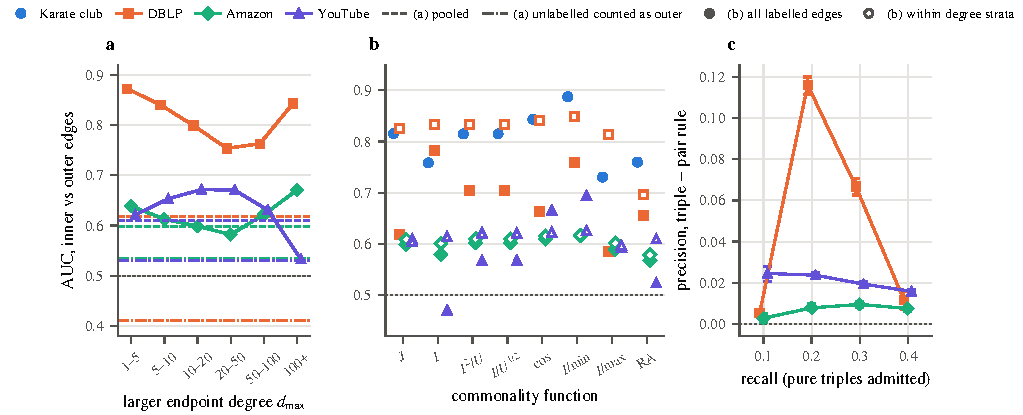
\includegraphics[width=\textwidth]{figures/fig_commonality.pdf}
  \caption{Commonality in networks with recorded memberships. (a)~AUC of
  closed-neighbourhood Jaccard for inner against outer edges within strata of $d_{\max}$
  (points), pooled (dashed), and with unlabelled edges counted as outer (dash-dotted), as
  in Ref.~\cite{deinega2023thesis}; the karate club is too small to stratify. (b)~AUC of
  eight functions over all labelled edges (filled) and within strata of both endpoint
  degrees (open). (c)~Precision of the triple minus the pair rule at equal recall, with
  95\% intervals from resampling the triples.}
  \label{fig:realcommonality}
\end{figure*}

% ---------------------------------------------------------------------------
\section{The method}
\label{sec:method}
% ---------------------------------------------------------------------------

HyperCommon has two settings: the commonality function $f$, which scores a pair of
nodes (closed-neighbourhood Jaccard unless stated otherwise), and the threshold $t$.
Given a graph $G$:
\begin{enumerate}
\item For every wedge $\{i,j,\ell\}$ -- three nodes, one adjacent to the other two,
  each counted once whether open or closed -- compute $f$ on its three pairs.
\item Admit the wedge as a hyperedge if all three values are at least $t$.
\item Join two admitted triples when they share two nodes, and return, for every
  connected component, the union of its triples' nodes.
\end{enumerate}
Commonality values are memoised per pair, and components are found on the bipartite
incidence graph between admitted triples and the pairs they contain, which has the
same triple components as the two-node-overlap graph and is linear in the number of
triples. Because the triple scores $s(T)=\min f$ over the pairs of $T$ do not depend on
$t$, the covers for every threshold follow from a single enumeration, each at the cost
of one component search. The threshold can be set from the graph alone, by maximising
the overlapping modularity of the cover~\cite{shen2009detect} (Sec.~\ref{sec:protocols}).
A local variant grows the community of a given seed triple by breadth-first search over
shared pairs, reading only the neighbourhoods of the nodes it reaches and of the
candidates it examines (Proposition~\ref{prop:local}).

\begin{figure*}[t]
  \centering
  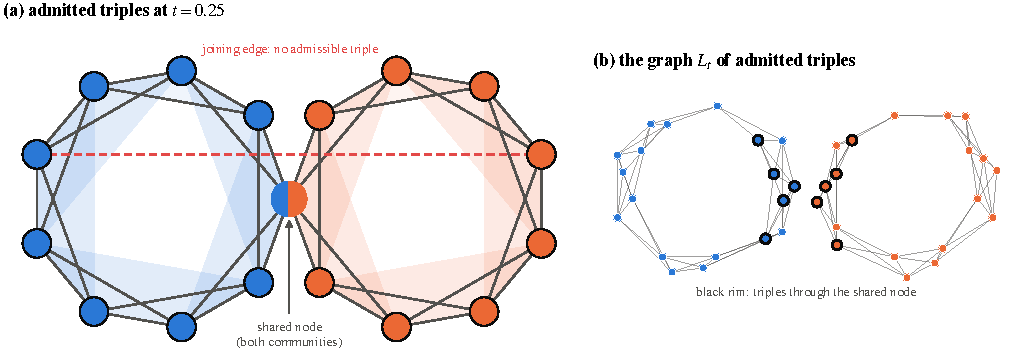
\includegraphics[width=0.85\textwidth]{figures/fig_schematic.pdf}
  \caption{The method on a toy graph, computed by the implementation. (a)~Two ring
  lattices of nine nodes ($k=4$) share one node, and one edge, placed by hand for the
  illustration between two nodes far from the shared node (it closes no triangle with
  it), joins them. Shaded triangles are the triples admitted at $t=0.25$, coloured by
  component; the shared node is admitted in both, the joining edge in none. (b)~The
  graph of admitted triples, linked when they share a pair ($L_t$), each component drawn
  on its own circle; its two components are the two communities. The rings have
  $s=9<2k+2$, outside the stated hypothesis of Theorem~\ref{thm:window} but within the
  ring sizes for which its window still holds (Sec.~\ref{app:proofsmore}).}
  \label{fig:schematic}
\end{figure*}

Figure~\ref{fig:schematic} illustrates the construction. Nodes in no admitted triple
remain unassigned, and communities have at least three members: the method reports only
what local evidence supports (coverage in Table~\ref{tab:S-coverage-label-free} of the
Supplemental Material~\cite{supplement}).

% ---------------------------------------------------------------------------
\section{Properties of the commonality hypergraph}
\label{sec:theory}
% ---------------------------------------------------------------------------

Throughout, $G=(V,E)$ is a finite simple undirected graph, $N[u]=\{u\}\cup N(u)$ is
the closed neighbourhood of $u$, and
\begin{equation}
  J(u,v)=\frac{|N[u]\cap N[v]|}{|N[u]\cup N[v]|}
  \label{eq:jaccard}
\end{equation}
is the commonality of the pair. A set $T=\{i,j,\ell\}$ of three distinct nodes is a
\emph{wedge} if one of its nodes is adjacent to the other two, and it is
\emph{admissible at threshold $t$} if it is a wedge and $J\ge t$ for all three of its
pairs. The admissible triples $\mathcal T_t$ are the hyperedges of a 3-uniform
hypergraph $\mathcal H_t=(V,\mathcal T_t)$. Let $L_t$ be its two-node-overlap graph,
whose vertices are the triples of $\mathcal T_t$, two of them adjacent when they share
exactly two nodes. The communities at threshold $t$ are the node sets of its
components:
\begin{equation}
  \mathcal C_t=\Bigl(\textstyle\bigcup_{T\in K}T\Bigr)_{K \text{ a connected component of } L_t}.
  \label{eq:communities}
\end{equation}
A node belongs to every community whose component contains a triple through it, so
$\mathcal C_t$ is a cover, and nodes in no admissible triple are left unassigned. All
results except Lemma~\ref{lem:ringJ} and Theorem~\ref{thm:window}, which are specific to
Jaccard, hold for any commonality function; proofs are in Appendix~\ref{app:proofs}.

\subsection{Determinism, locality and nesting}

\begin{proposition}[Order independence]
\label{prop:determinism}
$\mathcal C_t$ is a function of $(G,t)$ alone: it does not depend on a processing
order, a random seed, or the order in which triples are discovered.
\end{proposition}
This is the property the original formulation~\cite{deinega2023thesis} lacked: it
deleted each edge once used, so whether a later triple could still be formed depended on
which community had been grown first.

\begin{proposition}[Local query]
\label{prop:local}
Let $T_0\in\mathcal T_t$. Breadth-first search over $L_t$ from $T_0$, in which a
frontier pair $\{x,y\}$ is extended by every $w\in N(x)\cup N(y)$ with
$\{x,y,w\}\in\mathcal T_t$, visits exactly the component of $L_t$ that contains $T_0$,
and evaluates $J$ only on pairs within the closed neighbourhoods of the nodes it
reaches.
\end{proposition}

\begin{theorem}[Nesting]
\label{thm:nesting}
If $t_1\le t_2$, then $L_{t_2}$ is the subgraph of $L_{t_1}$ induced on
$\mathcal T_{t_2}$, and every community of $\mathcal C_{t_2}$ is contained in a
community of $\mathcal C_{t_1}$.
\end{theorem}
Raising $t$ only splits communities or removes nodes; it never merges two of them. The
covers at all thresholds therefore form one hierarchy, which changes only at the
finitely many values $J$ takes. Its two ends carry no information: on a connected graph
the cover at $t=0$ is one community, and at $t=1$ only classes of nodes with identical
closed neighbourhoods remain, so the most accurate threshold is interior
(Proposition~\ref{prop:endpoints} of the Supplemental Material).

\subsection{Exact recovery on overlapping ring lattices}

Consider $r$ rings of sizes $s_i\ge 2k+2$, each node joined to its $k/2$ nearest
neighbours on either side ($k\ge4$ even), and a set of \emph{merges}: a node $v$ of one
ring is absorbed into a node $u$ of another, which inherits $v$'s edges and so belongs
to both ground-truth communities. The merges are \emph{isolated} if each original node
takes part in at most one merge and, on each original ring, any two merge positions are
more than $k$ apart.

\begin{lemma}[Commonality on the lattice]
\label{lem:ringJ}
With isolated merges, let $x,y$ be unmerged nodes at ring distance $d\le k$, $u$ a
merged node at distance $d$ from $x$ along one of its rings, and $z,y'$ neighbours of
$u$ on its two different rings. Then
\begin{equation}
\begin{aligned}
  J(x,y)&=J(d)\equiv\frac{k+1-d}{k+1+d},\\
  J(u,x)&=J_u(d)\equiv\frac{k+1-d}{2k+1+d},\\
  J(z,y')&=\frac{1}{2k+1},
\end{aligned}
  \label{eq:ringJ}
\end{equation}
and every other pair on distinct rings has $J=0$.
\end{lemma}

\begin{theorem}[Exact recovery window]
\label{thm:window}
With at least one merge, all of them isolated, $\mathcal C_t$ equals the ground truth
if and only if
\begin{equation}
\begin{aligned}
  &\frac{1}{2k+1}<t\le t^{+}(k),\\
  &t^{+}(k)\equiv\min\Bigl\{J_u(1),\,\max\bigl(J(3),J_u(2)\bigr)\Bigr\}\\
  &\phantom{t^{+}(k)}=\min\Bigl\{\frac{k}{2k+2},\,\max\Bigl(\frac{k-2}{k+4},\frac{k-1}{2k+3}\Bigr)\Bigr\}.
\end{aligned}
  \label{eq:window}
\end{equation}
Without merges the condition is $0\le t\le J(2)=(k-1)/(k+3)$.
\end{theorem}

Explicitly, $t^{+}(k)=k/(2k+2)$ for $k\ge8$, so the window widens towards $(0,\tfrac12)$
as $k$ grows: $(1/17,4/9]$ for $k=8$ and $(1/33,8/17]$ for $k=16$. Both edges have a
direct reading. The lower edge is the price of overlap: a shared node is the only bridge
between its two rings, and the bridge is cut once $t$ exceeds the commonality $1/(2k+1)$
of the rings' members across it. The upper edge is set by the shared nodes themselves:
their commonality with either ring is roughly halved by their double membership, and
above it they drop out. For one isolated merge between rings of degrees $k_a$ and $k_b$
the same argument gives
\begin{equation}
\begin{aligned}
  &\frac{1}{k_a+k_b+1}<t\le\min\{U(k_a,k_b),U(k_b,k_a)\},\\
  &U(x,y)=\min\Bigl\{\frac{x}{x+y+2},\,\max\Bigl(\frac{x-2}{x+4},\frac{x-1}{x+y+3}\Bigr)\Bigr\},
\end{aligned}
  \label{eq:windowab}
\end{equation}
and a family with several merge types is recovered exactly if and only if $t$ lies in the
intersection of their windows; once $k_a\ge2k_b^2-2$ the windows of dense--sparse and
sparse--sparse merges are disjoint, and no single threshold recovers a family with
both. We verified these windows exactly, in rational arithmetic, for $k=4,\dots,24$ and
eleven degree pairs, together with the smaller-ring and multi-ring cases of
Sec.~\ref{app:proofsmore} of the Supplemental Material.

\begin{proposition}[Shared pairs]
\label{prop:sharedpairs}
Let $A$ and $B$ be ground-truth communities, and let the pair $\{u_1,u_2\}\subseteq
A\cap B$ lie in an admissible triple $T_A\subseteq A$ and in an admissible triple
$T_B\subseteq B$. Then $T_A$ and $T_B$ lie in the same component of $L_t$, whatever the
commonality between $A\setminus B$ and $B\setminus A$.
\end{proposition}
Two communities that share a pair of nearby nodes are thus read as one, much as
$k$-clique percolation reads communities sharing $k-1$ nodes as
one~\cite{palla2005uncovering}. The random merges of our benchmarks are not isolated:
with $o_n=0.05$, between $6\%$ and $61\%$ of the rings of a family are fused with
another just above the lower edge of the window (Table~\ref{tab:doublebonds}).

\begin{corollary}[Pair-disjointness]
\label{cor:pairdisjoint}
At every threshold $t$, all admissible triples that contain a given pair of nodes lie in
one component of $L_t$. In particular, an edge that lies in an admissible triple is
assigned to exactly one community, and the communities of a node are those of the
admitted edges incident to it.
\end{corollary}
No pair of nodes binds two communities, so a node's memberships can be read off its
admitted edges, as in link communities~\cite{ahn2010link,evans2009line}. This shares an
assumption of clique percolation and link clustering that ground truth contradicts in
many social and collaboration networks, where overlaps are more densely connected than
the rest of the communities~\cite{yang2014structure,yang2012community}; in co-purchasing
networks, by contrast, overlaps are small~\cite{yang2014overlapping}.

\subsection{Cost}
\label{sec:cost}

Admissibility is decided for each of the $W=\sum_v\binom{d_v}{2}$ wedges from three pair
commonalities, all counted in one pass over the wedges, so the time and memory are
\begin{equation}
  O(n+m+W)=O\bigl(n[1+\langle d^2\rangle]\bigr)
  \label{eq:cost}
\end{equation}
for $n$ nodes and $m$ edges. For a power-law degree tail of exponent $\gamma$ this is
$O(n)$ when $\gamma>3$ and $O(n+m\log m)$ at $\gamma=3$, the exponent of the
Barab\'asi--Albert model~\cite{albert2002statistical}; for $2<\gamma<3$ it grows as a
power of $n$ set by the largest degree, and how often real tails are that heavy is
debated~\cite{broido2019scale,voitalov2019scale}.

In practice the heavy tail matters less than $W$ suggests. Since
$J(u,v)\le\rho(u,v)\equiv(\min(d_u,d_v)+1)/(\max(d_u,d_v)+1)$, a wedge containing an edge
with $\rho<t_{\min}$ cannot be admitted at any $t\ge t_{\min}$ and can be discarded
before scoring, provided the remaining commonalities are computed from the complete
neighbourhoods (Sec.~\ref{app:proofsmore}). The excess wedges of a heavy tail are exactly
of this kind: they join a hub to neighbours of far smaller degree. On thirty-two SNAP
networks with up to $4\times10^6$ nodes, $W/(m\ln m)$ ranges from $0.15$ on road networks
to $268$ on a web graph with hubs of degree $8.4\times10^4$, but after pruning at
$t_{\min}=0.02$ it is at most $12$ on all of them (Table~\ref{tab:S-wedges}); on YouTube
it falls from $33$ to $3.7$. The cost is therefore that of the $\gamma=3$ case even where
$W$ itself is not. Once the triple scores are stored, every further threshold costs
$O(W)$, so a whole sweep of the threshold costs one scoring, whereas a sweep of Leiden's
resolution or Infomap's Markov time costs a full run per value. Clique percolation is the
costly method: the number of maximal cliques can grow exponentially with
$n$~\cite{moon1965cliques}, and on one of the fourteen smaller networks of
Sec.~\ref{sec:real} it is out of reach.

% ---------------------------------------------------------------------------
\section{Benchmarks and evaluation protocol}
\label{sec:protocol}
% ---------------------------------------------------------------------------

\subsection{Benchmarks}
\label{sec:benchmarks}

\emph{Planted overlapping ring lattices.} Following
Refs.~\cite{watts1998collective,kanovsky2010small}, each planted community is a ring
lattice of $s$ nodes and degree $k$, and communities may differ in $s$ and $k$. Overlap is
planted by merging $\lfloor o_n n_0\rfloor$ pairs of nodes from different rings ($n_0$
nodes before the merges); the survivor belongs to both rings and keeps both
neighbourhoods. Noise rewires a fraction $p\in\{0,0.05,\dots,0.8\}$ of the original
edges, each keeping one endpoint and moving the other to a non-neighbour chosen
uniformly or preferentially. The families (Table~\ref{tab:shapes}) range from uniform
rings ($n_0=2000$, $(s,k)\in\{(50,8),(100,16)\}$) through ``two worlds'' (five dense rings
of 200 nodes, twenty sparse rings of 50) and ``three big, many small'' to a gradient of
ten rings from 600 to 30 nodes; at $o_n\in\{0,0.05,0.10\}$, with four settings under
preferential noise, they give 28 ring settings. Numbers quoted for a family without its overlap level
are at $o_n=0.05$. Further families each isolate one question: \emph{isolated-merge}
families place the merges within the hypothesis of Theorem~\ref{thm:window};
\emph{geometry} families rewire a fraction $q$ of each ring's edges inside the ring,
moving each community from a lattice ($q=0$) to a random graph ($q=1$) at fixed sizes,
degrees and overlap; and controls add hubs, split the edges of shared nodes between
their rings as in LFR graphs, use random geometric communities, or have no planted
communities at all (a random geometric graph and a Holme--Kim
graph~\cite{holme2002growing}). Every setting is in Sec.~\ref{app:design} of the
Supplemental Material.

\emph{Overlapping LFR graphs.} We use the reference
generator~\cite{lancichinetti2008benchmark,lancichinetti2009benchmarks} with $N=2000$, a
fraction $o_n\in\{0,0.1,0.3\}$ of nodes in $o_m=2$ communities and mixing
$\mu\in\{0.1,\dots,0.6\}$, plus five families at $o_n=0.1$ that change the degree, $o_m$,
the community sizes or the clustering.

\subsection{Methods compared}
\label{sec:methods}

Three \emph{ablations} each remove one ingredient: \emph{triangles only} admits only
closed triples (J-thresholded 3-clique percolation); \emph{two-test} admits an open
wedge when its two edges pass, without testing its non-adjacent pair; and
\emph{edge-connected} joins triples only through shared edges. The fourteen other
methods are link communities~\cite{ahn2010link} with the same similarity, cut at every
value of HyperCommon's threshold grid; clique percolation
(CPM)~\cite{palla2005uncovering}; SCAN~\cite{xu2007scan} with cosine and with Jaccard
similarity (SCAN-J); Leiden~\cite{traag2019leiden} with the Reichardt--Bornholdt
modularity~\cite{reichardt2006statistical} and with the Constant Potts
Model~\cite{traag2011narrow} (L-CPM); Infomap~\cite{rosvall2008maps} over a range of
Markov times~\cite{schaub2012markov,kheirkhahzadeh2016efficient};
Walktrap~\cite{pons2006walktrap}; label propagation (LPA)~\cite{raghavan2007near};
SLPA~\cite{xie2011slpa}; DEMON~\cite{coscia2012demon}; ANGEL~\cite{rossetti2020angel};
OSLOM~\cite{lancichinetti2011finding}, which keeps a group only if it is significant
against a configuration-model null, with its significance level as the parameter; and
the nested degree-corrected stochastic block model (SBM)~\cite{peixoto2014hierarchical},
fitted with \textsc{graph-tool}~\cite{peixoto_graphtool}, each level of its hierarchy
treated as a parameter value. OSLOM and the SBM were run on the ring and LFR benchmarks,
the random-geometric controls and the null graphs, and OSLOM also on all real networks.
BigClam~\cite{yang2013overlapping}, ego-splitting~\cite{epasto2017ego} and the
local-fitness method LFM~\cite{lancichinetti2009lfm} are not included (LFM took more than
ten minutes on a single 2000-node graph, against the thousands of graphs of the
benchmark). Every grid (Table~\ref{tab:grids}) was widened and fixed after a preliminary
run and before any reported result was computed.

\subsection{Protocols}
\label{sec:protocols}

Every method, HyperCommon included, is scored under the same rules. \emph{Oracle}: on
each test graph each method is credited with its best parameter, which measures what
its family of covers can achieve. \emph{Label-free}: each method takes the parameter
whose cover has the largest overlapping modularity~\cite{shen2009detect},
\begin{equation}
  Q_{\rm ov}=\frac{1}{2m}\sum_{c}\sum_{u,v\in c}\frac{1}{O_uO_v}
  \Bigl(A_{uv}-\frac{d_ud_v}{2m}\Bigr),
  \label{eq:qov}
\end{equation}
where $O_u$ is the number of communities that contain $u$ and nodes in no community
contribute nothing; for a partition this is the Newman--Girvan modularity. Two further
protocols check these two: \emph{native}, each method at its own default or selection
rule where it has one (Leiden at $\gamma=1$, L-CPM at the edge density, link communities
at the largest partition density, Infomap at Markov time 1, SLPA at $r=0.1$, OSLOM at its
default level $0.1$, the SBM at its finest level), and \emph{frozen}, one parameter per
family and method fixed on separate calibration graphs.

\subsection{Metrics}
\label{sec:metrics}

Covers are compared with the Omega index~\cite{collins1988omega}. For a cover
$\mathcal C$ let $c_{\mathcal C}(i,j)$ be the number of its communities containing both
$i$ and $j$, and $\pi_{\mathcal C}(c)$ the fraction of pairs with $c_{\mathcal C}=c$;
with ground truth $\mathcal G$, $\Omega=(\Omega_u-\Omega_e)/(1-\Omega_e)$, where
$\Omega_u=\Pr[c_{\mathcal C}=c_{\mathcal G}]$ and
$\Omega_e=\sum_c\pi_{\mathcal C}(c)\pi_{\mathcal G}(c)$. Omega counts node pairs and is
dominated by the largest communities, so we also report the overlapping normalised
mutual information (ONMI)~\cite{mcdaid2011normalized}, a per-community recovery score
(the mean Jaccard similarity of each true community with its best match), the best-match
F1 score~\cite{yang2015defining} on real networks, and coverage. Unassigned nodes are
penalised by Omega and ONMI. Each metric is averaged over the noise range per test seed;
uncertainties are 95\% bootstrap intervals over ten test seeds, and differences between
methods are paired by seed.

% ---------------------------------------------------------------------------
\section{Results}
\label{sec:results}
% ---------------------------------------------------------------------------

\subsection{Exact recovery and the threshold}
\label{sec:recovery}

An exact implementation confirms Theorem~\ref{thm:window}. On rings whose merges satisfy
its isolation hypothesis ($n_0=2000$, $o_n=0.01$), without noise HyperCommon returns the
planted rings exactly at each of the 20 thresholds of our grid inside the window for
$k=8$ and the 22 inside it for $k=16$, and at no threshold outside it ($\Omega<0.98$).
With a fifth of the edges rewired, the mean $\Omega$ at the best threshold is still
$1.000$ for $k=16$ and $0.991$ for $k=8$. Without the third-pair test the same graphs
are never recovered exactly: the two edges of the wedge that crosses a merge have
commonality $J_u(1)$, at least every threshold of the window, so the pair rule admits
that wedge throughout it.

\begin{figure*}[t]
  \centering
  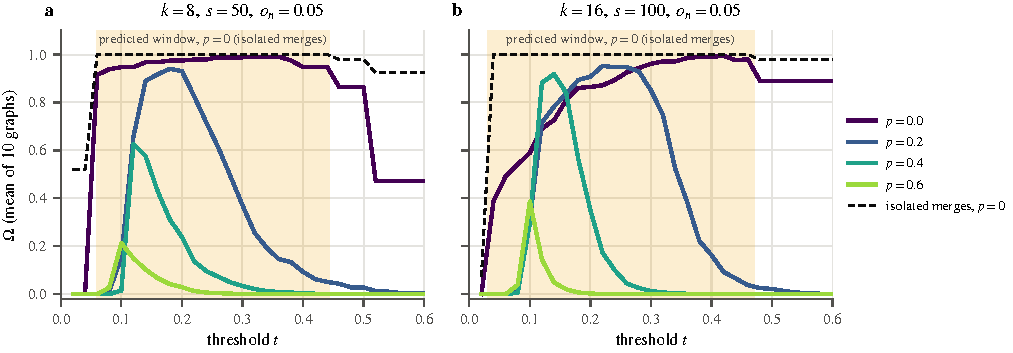
\includegraphics[width=\textwidth]{figures/fig_omega_t.pdf}
  \caption{Accuracy of HyperCommon as a function of the threshold on overlapping
  uniform rings ($n_0=2000$, $o_n=0.05$), one curve per rewiring level $p$, each the mean
  over ten test graphs. Shaded: the exact-recovery window that
  Theorem~\ref{thm:window} predicts for $p=0$ when merges are isolated; the plotted
  graphs' random merges do not satisfy the isolation hypothesis. Black dashed: graphs
  with isolated merges ($o_n=0.01$, merges more than $2k$ apart) at $p=0$, which reach
  $\Omega=1$ at every grid threshold inside the window and at none outside it.}
  \label{fig:omegat}
\end{figure*}

When merges fall at random they are rarely isolated: at $o_n=0.05$ a ring carries on
average at least as many merge positions as fit on it more than $k$ apart, and rings fuse through
nearby merged nodes (Proposition~\ref{prop:sharedpairs}). The noise-free curve still
stays between $0.92$ and $0.99$ across the window for $k=8$ [Fig.~\ref{fig:omegat}(a)].
As noise grows the best threshold moves down towards $t\approx0.1$, so the threshold has
to be chosen per graph. The overlapping modularity of the cover chooses it well: the
label-free threshold attains at least $95\%$ of the best threshold's mean $\Omega$ on 27
of the 36 benchmark settings and at least $90\%$ on 31 (Tables~\ref{tab:labelfree}
and~\ref{tab:oracle}).

\subsection{Planted rings}
\label{sec:planted}

\begin{table*}[t]
\caption{Scorecard of the benchmarks under the four protocols: $\Omega$ of HyperCommon minus that of the best other method (ablations excluded), mean over the noise range ($p\in[0,0.8]$ for rings, $\mu\in[0.1,0.6]$ for LFR), ten test graphs per noise level, with the best other method in brackets when HyperCommon is not significantly ahead of it and its difference rounds to 0.00 or below. Mark: the paired 95\% bootstrap interval of the difference over the ten test seeds lies above zero ($+$), contains zero ($=$) or lies below zero ($-$); intervals and the second-best method in Table~\ref{tab:S-intervals}. Oracle: best parameter per graph; label-free: largest overlapping modularity, Eq.~\eqref{eq:qov}; frozen: one parameter per family from calibration graphs; native: each method's own default or selection rule where it has one (Sec.~\ref{sec:protocol}), the label-free choice otherwise. Counts are not corrected for multiplicity. Method abbreviations as in Table~\ref{tab:labelfree}; the full tables are Tables~\ref{tab:labelfree} and~\ref{tab:oracle}--\ref{tab:native}.}
\label{tab:scorecard}
\scriptsize\setlength{\tabcolsep}{3pt}
\begin{ruledtabular}
\begin{tabular}{llcccc}
Family & $o_n$ & oracle & label-free & frozen & native \\
\hline
uniform, $k{=}8$ & 0.00 & $-0.05^{-}$ (Leiden) & $-0.00^{=}$ (Leiden) & $-0.08^{-}$ (Leiden) & $-0.00^{=}$ (Leiden) \\
 & 0.05 & $+0.00^{+}$ & $+0.02^{+}$ & $-0.03^{-}$ (Leiden) & $+0.06^{+}$ \\
 & 0.10 & $+0.01^{+}$ & $+0.05^{+}$ & $+0.01^{=}$ & $+0.06^{+}$ \\
\hline
uniform, $k{=}16$ & 0.00 & $-0.08^{-}$ (Leiden) & $-0.06^{-}$ (Leiden) & $-0.10^{-}$ (Leiden) & $-0.06^{-}$ (Leiden) \\
 & 0.05 & $-0.04^{-}$ (Leiden) & $-0.03^{-}$ (Leiden) & $-0.19^{-}$ (Leiden) & $-0.04^{-}$ (Leiden) \\
 & 0.10 & $-0.01^{=}$ (Leiden) & $+0.00^{=}$ (Leiden) & $-0.32^{-}$ (Leiden) & $+0.00^{=}$ (Leiden) \\
\hline
equal $k$, unequal $s$, $k{=}8$ & 0.00 & $-0.03^{-}$ (Leiden) & $+0.01^{+}$ & $-0.04^{-}$ (Leiden) & $+0.01^{+}$ \\
 & 0.05 & $+0.01^{+}$ & $+0.03^{+}$ & $+0.00^{=}$ (Link) & $+0.09^{+}$ \\
 & 0.10 & $+0.00^{=}$ (Link) & $+0.04^{+}$ & $+0.00^{=}$ (CPM) & $+0.08^{+}$ \\
\hline
equal $k$, unequal $s$, $k{=}16$ & 0.00 & $-0.07^{-}$ (Leiden) & $-0.04^{-}$ (Leiden) & $-0.10^{-}$ (Leiden) & $-0.04^{-}$ (Leiden) \\
 & 0.05 & $-0.04^{-}$ (Leiden) & $+0.00^{=}$ (Leiden) & $-0.17^{-}$ (Leiden) & $+0.01^{+}$ \\
 & 0.10 & $+0.01^{+}$ & $+0.04^{+}$ & $-0.31^{-}$ (Leiden) & $+0.04^{+}$ \\
\hline
equal $s$, unequal $k$ & 0.00 & $-0.03^{-}$ (Leiden) & $-0.01^{=}$ (L-CPM) & $-0.07^{-}$ (Leiden) & $+0.00^{=}$ (Leiden) \\
 & 0.05 & $-0.01^{-}$ (L-CPM) & $-0.01^{=}$ (L-CPM) & $-0.18^{-}$ (Leiden) & $+0.02^{+}$ \\
 & 0.10 & $-0.03^{-}$ (L-CPM) & $-0.02^{-}$ (L-CPM) & $-0.33^{-}$ (L-CPM) & $+0.03^{+}$ \\
\hline
two worlds & 0.00 & $-0.00^{-}$ (L-CPM) & $+0.03^{+}$ & $-0.05^{-}$ (L-CPM) & $+0.01^{+}$ \\
 & 0.05 & $-0.01^{-}$ (L-CPM) & $+0.10^{+}$ & $-0.25^{-}$ (L-CPM) & $+0.00^{=}$ (L-CPM) \\
 & 0.10 & $-0.00^{=}$ (L-CPM) & $+0.06^{+}$ & $-0.38^{-}$ (L-CPM) & $+0.01^{=}$ \\
\hline
three big, many small & 0.00 & $+0.01^{+}$ & $+0.03^{+}$ & $+0.03^{+}$ & $+0.09^{+}$ \\
 & 0.05 & $+0.07^{+}$ & $+0.10^{+}$ & $-0.16^{-}$ (CPM) & $+0.10^{+}$ \\
 & 0.10 & $+0.04^{+}$ & $+0.06^{+}$ & $-0.23^{-}$ (CPM) & $+0.06^{+}$ \\
\hline
gradient & 0.00 & $-0.01^{-}$ (Link) & $-0.19^{-}$ (Link) & $-0.00^{=}$ (Link) & $-0.14^{-}$ (CPM) \\
 & 0.05 & $+0.03^{+}$ & $-0.16^{-}$ (Link) & $-0.02^{=}$ (ANGEL) & $-0.11^{-}$ (ANGEL) \\
 & 0.10 & $+0.03^{+}$ & $-0.15^{-}$ (Link) & $-0.14^{-}$ (DEMON) & $-0.12^{-}$ (CPM) \\
\hline
uniform $k{=}8$, $\alpha{=}1$ & 0.05 & $+0.01^{+}$ & $+0.04^{+}$ & $-0.03^{-}$ (Leiden) & $+0.08^{+}$ \\
uniform $k{=}8$, $\alpha{=}2$ & 0.05 & $+0.01^{+}$ & $+0.02^{+}$ & $-0.02^{-}$ (Leiden) & $+0.08^{+}$ \\
two worlds, $\alpha{=}1$ & 0.05 & $-0.05^{-}$ (L-CPM) & $+0.11^{+}$ & $-0.29^{-}$ (L-CPM) & $+0.12^{+}$ \\
two worlds, $\alpha{=}2$ & 0.05 & $+0.00^{=}$ (L-CPM) & $+0.13^{+}$ & $-0.20^{-}$ (L-CPM) & $+0.15^{+}$ \\
\hline
LFR, $o_n{=}0$ &  & $-0.14^{-}$ (Leiden) & $-0.16^{-}$ (Info.) & $-0.18^{-}$ (Leiden) & $-0.16^{-}$ (Info.) \\
LFR, $o_n{=}0.1$ &  & $-0.15^{-}$ (L-CPM) & $-0.18^{-}$ (Info.) & $-0.24^{-}$ (Info.) & $-0.19^{-}$ (Info.) \\
LFR, $o_n{=}0.3$ &  & $-0.21^{-}$ (SLPA) & $-0.19^{-}$ (Info.) & $-0.40^{-}$ (Leiden) & $-0.21^{-}$ (SLPA) \\
LFR, $\langle k\rangle{=}10$ &  & $-0.33^{-}$ (Leiden) & $-0.28^{-}$ (Info.) & $-0.37^{-}$ (Leiden) & $-0.28^{-}$ (Info.) \\
LFR, $o_m{=}4$ &  & $-0.15^{-}$ (SLPA) & $-0.09^{-}$ (Info.) & $-0.18^{-}$ (SLPA) & $-0.10^{-}$ (SLPA) \\
LFR, sizes 50--250 &  & $-0.45^{-}$ (Leiden) & $-0.45^{-}$ (Leiden) & $-0.55^{-}$ (Leiden) & $-0.43^{-}$ (Leiden) \\
LFR, $C_{\rm LFR}{=}0.3$ &  & $-0.23^{-}$ (Leiden) & $-0.23^{-}$ (SLPA) & $-0.31^{-}$ (Leiden) & $-0.25^{-}$ (SLPA) \\
LFR, $C_{\rm LFR}{=}0.5$ &  & $-0.08^{-}$ (Leiden) & $-0.11^{-}$ (LPA) & $-0.14^{-}$ (SLPA) & $-0.12^{-}$ (SLPA) \\
\hline
$+/{=}/-$, rings & & 11/4/13 of 28 & 16/5/7 of 28 & 1/5/22 of 28 & 17/5/6 of 28 \\
$+/{=}/-$, LFR & & 0/0/8 of 8 & 0/0/8 of 8 & 0/0/8 of 8 & 0/0/8 of 8 \\
\end{tabular}
\end{ruledtabular}
\end{table*}


\begin{figure*}[t]
  \centering
  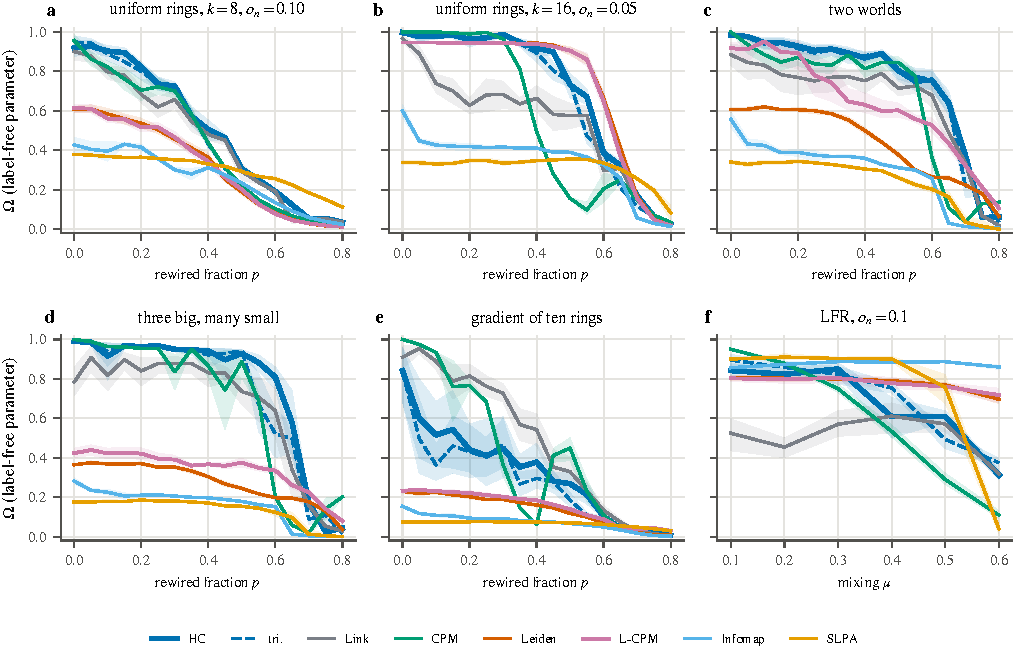
\includegraphics[width=\textwidth]{figures/fig_benchmarks.pdf}
  \caption{Accuracy against noise with every method's parameter chosen without labels
  (largest overlapping modularity on each graph); lines are means over ten test graphs
  and bands 95\% bootstrap intervals. (a,b)~Uniform rings; (c--e)~rings of unequal size
  and density ($o_n=0.05$); (f)~overlapping LFR graphs, against the mixing parameter. In
  (e) the selector picks too fine a cover for HyperCommon (Sec.~\ref{sec:planted}).
  OSLOM and the stochastic block model are not drawn; on the family of (f) OSLOM is the
  most accurate method (Table~\ref{tab:labelfree}). The same panels under the oracle
  protocol are in Fig.~\ref{fig:benchmarksoracle}.}
  \label{fig:benchmarks}
\end{figure*}

Table~\ref{tab:scorecard} summarises the benchmarks. Without labels, over the 28 ring
settings HyperCommon has the highest $\Omega$ in 15, by paired 95\% intervals that
exclude zero, is level with the best other method in 6 and trails in 7: on dense rings
with little overlap, where Leiden leads ($0.84$ against $0.78$ at $k=16$, $o_n=0$), on
rings of equal size and unequal degree at $o_n=0.10$, and on the gradient, where link
communities lead. The margins are largest where community sizes differ and communities
overlap: $\Omega=0.78$ against $0.68$ for clique percolation on three big, many small,
and $0.76$ against $0.66$ on two worlds [Fig.~\ref{fig:benchmarks}(c,d)].

Part of these margins lies in the selector rather than in the objectives. At its best
resolution the Constant Potts Model reaches $0.71$ on three big, many small and $0.78$ on
two worlds, against $0.34$ and $0.64$ when modularity chooses its resolution, while
HyperCommon goes from $0.80$ to $0.78$ and from $0.78$ to $0.76$. Two checks bound this
effect. At each method's own default or selection rule (native protocol), HyperCommon
is still ahead in 17 of the 28 settings, although the Constant Potts Model at the edge
density is then level with it on two worlds with overlap. With the best parameter on
every graph (oracle), every method narrows the gap: HyperCommon is ahead in 11, level in
4 and behind in 13, mostly behind one of the two Leiden objectives, and stays ahead on
three big, many small at every overlap level ($0.80$ against $0.72$ for link communities)
and on the gradient with overlap. Modularity with a single resolution fails on the
gradient even without noise ($\Omega=0.28$ for Leiden, against $0.99$ for HyperCommon),
because small rings are merged while large ones are
split~\cite{fortunato2007resolution,lancichinetti2011limits}. With one parameter frozen
per family, HyperCommon leads in only 1 setting: its best threshold moves with noise, so
one threshold fits the noise-free graphs or the noisy ones but not both. On the gradient
the label-free selector errs the other way, picking too fine a cover ($181$ communities
against $147$ at the best threshold and $10$ planted).

Omega is dominated by the largest communities. On two worlds and three big, many small,
HyperCommon recovers the large rings best but splits the small sparse ones, which the
Constant Potts Model recovers best ($0.53$--$0.54$ against $0.33$--$0.38$;
Tables~\ref{tab:recsmall} and~\ref{tab:reclarge}), so with labels the Constant Potts
Model leads there by ONMI. Over the 28 ring settings HyperCommon leads by ONMI on 10 with
labels and on 15 without (Tables~\ref{tab:onmi-oracle} and~\ref{tab:onmi-label-free}).
Without labels its accuracy also decays latest with noise, or within $0.01$ of the
latest, in ten of the sixteen ring families (Table~\ref{tab:robust}).

\subsection{Ablations}
\label{sec:ablations}

Testing the third, non-adjacent pair of a wedge matters most: without it $\Omega$ falls
in all 36 benchmark settings under the oracle and the label-free protocol, by
$0.06$--$0.34$ on rings and up to $0.42$ on LFR graphs, because a wedge whose two edges
pass reaches into another community whenever its centre has a neighbour there. Admitting
open wedges improves on triangles alone in 26 and 25 of the 36 settings under the two
protocols, most where triangles are scarce ($0.04$--$0.11$ on sparse rings). Joining
triples only through shared edges changes $\Omega$ by at most $0.02$ on the rings when the
parameter is chosen per graph and is slightly better on most LFR families; we keep
joins through non-adjacent pairs because they give Corollary~\ref{cor:pairdisjoint}.
Link communities, whose edge similarity is the commonality of the wedge's third pair,
are less accurate than HyperCommon in 25 of the 28 ring settings under both protocols;
the edge tests separate the two most where communities overlap. Among the commonality
functions, Jaccard is the best, or within $0.01$ of it, on seventeen of eighteen
benchmark settings with the best threshold (Tables~\ref{tab:familyoracle}
and~\ref{tab:familyfree}).

\subsection{Where it breaks: LFR graphs and random communities}
\label{sec:geometry}

\begin{table*}[t]
\caption{Internal geometry: before the noise, a fraction $q$ of each ring's edges is rewired inside the ring, from lattice rings ($q=0$) to rings that are random graphs ($q=1$), at fixed size and mean degree; $o_n=0.05$. Uniform: 40 rings of 50 nodes, $k=8$; two worlds: five rings of 200 nodes ($k=32$) and twenty of 50 ($k=8$); three big, many small: three of 400 ($k=32$) and sixteen of 50 ($k=8$); gradient: ten rings of 600 to 30 nodes ($k=16$ to 8). Mean $\Omega$ over $p\in\{0,0.1,\dots,0.6\}$, ten test graphs per noise level, under the oracle and label-free protocols, for HyperCommon (HC), its triangles-only variant and the best other method; $C$: mean clustering of the noiseless graphs (ten seeds); cov.: coverage of HC's label-free cover. Superscripts on HC: paired 95\% interval of its difference from the best other method excludes zero ($^+$ HC ahead, $^-$ behind). Bold: HC best or within 0.005 of the best other method. Means are over $p\in\{0,0.1,\dots,0.6\}$, so the $q=0$ entries differ from those of Tables~\ref{tab:labelfree} and~\ref{tab:oracle} for the same families, which average over $p\in[0,0.8]$.}
\label{tab:geometry}
\footnotesize\setlength{\tabcolsep}{3pt}
\begin{ruledtabular}
\begin{tabular}{lcccccccccc}
 & & & \multicolumn{3}{c}{oracle} & \multicolumn{4}{c}{label-free} \\
Family & $q$ & $C$ & HC & tri. & best other & HC & tri. & best other & cov. \\
\hline
uniform, $k{=}8$ & 0.0 & 0.62 & \textbf{0.73$^+$} & 0.65 & 0.73 (Link) & \textbf{0.70$^+$} & 0.64 & 0.67 (Link) & 0.98 \\
 & 0.1 & 0.48 & 0.68$^-$ & 0.56 & 0.81 (Leiden) & 0.65 & 0.56 & 0.66 (Leiden) & 0.97 \\
 & 0.3 & 0.28 & 0.62$^-$ & 0.41 & 0.85 (Leiden) & 0.57$^-$ & 0.41 & 0.74 (Infomap) & 0.95 \\
 & 0.6 & 0.16 & 0.61$^-$ & 0.28 & 0.86 (Leiden) & 0.55$^-$ & 0.28 & 0.77 (Infomap) & 0.96 \\
 & 1.0 & 0.15 & 0.60$^-$ & 0.29 & 0.85 (Leiden) & 0.55$^-$ & 0.28 & 0.78 (Infomap) & 0.95 \\
\hline
two worlds & 0.0 & 0.67 & \textbf{0.91} & 0.90 & 0.91 (L-CPM) & \textbf{0.89$^+$} & 0.89 & 0.82 (CPM) & 0.94 \\
 & 0.1 & 0.51 & 0.88$^-$ & 0.87 & 0.94 (L-CPM) & 0.86$^-$ & 0.86 & 0.91 (L-CPM) & 0.93 \\
 & 0.3 & 0.30 & 0.84$^-$ & 0.81 & 0.95 (L-CPM) & 0.82$^-$ & 0.80 & 0.92 (L-CPM) & 0.94 \\
 & 0.6 & 0.17 & 0.72$^-$ & 0.68 & 0.95 (L-CPM) & 0.69$^-$ & 0.66 & 0.92 (L-CPM) & 0.91 \\
 & 1.0 & 0.16 & 0.66$^-$ & 0.66 & 0.95 (L-CPM) & 0.62$^-$ & 0.66 & 0.92 (L-CPM) & 0.92 \\
\hline
three big, many small & 0.0 & 0.68 & \textbf{0.94$^+$} & 0.93 & 0.87 (CPM) & \textbf{0.93$^+$} & 0.91 & 0.85 (CPM) & 0.90 \\
 & 0.1 & 0.51 & 0.92$^-$ & 0.91 & 0.95 (L-CPM) & \textbf{0.91$^+$} & 0.91 & 0.83 (CPM) & 0.91 \\
 & 0.3 & 0.28 & 0.84$^-$ & 0.80 & 0.96 (L-CPM) & 0.83$^-$ & 0.79 & 0.95 (L-CPM) & 0.91 \\
 & 0.6 & 0.13 & 0.51$^-$ & 0.61 & 0.96 (L-CPM) & 0.50$^-$ & 0.56 & 0.95 (L-CPM) & 0.83 \\
 & 1.0 & 0.11 & 0.28$^-$ & 0.54 & 0.96 (L-CPM) & 0.27$^-$ & 0.45 & 0.95 (L-CPM) & 0.80 \\
\hline
gradient of ten rings & 0.0 & 0.66 & \textbf{0.74$^+$} & 0.72 & 0.70 (Link) & 0.42$^-$ & 0.37 & 0.64 (Link) & 0.93 \\
 & 0.1 & 0.49 & 0.65$^-$ & 0.63 & 0.73 (L-CPM) & 0.43$^-$ & 0.38 & 0.55 (Link) & 0.93 \\
 & 0.3 & 0.25 & 0.44$^-$ & 0.43 & 0.86 (L-CPM) & 0.40$^-$ & 0.34 & 0.76 (Walktrap) & 0.93 \\
 & 0.6 & 0.08 & 0.16$^-$ & 0.11 & 0.88 (L-CPM) & 0.16$^-$ & 0.09 & 0.86 (L-CPM) & 0.87 \\
 & 1.0 & 0.04 & 0.11$^-$ & 0.02 & 0.87 (L-CPM) & 0.09$^-$ & 0.01 & 0.85 (L-CPM) & 0.89 \\
\end{tabular}
\end{ruledtabular}
\end{table*}


HyperCommon trails on all eight LFR families under every protocol; OSLOM is the most
accurate method on most of them without labels. The pairwise signal is not what fails:
the AUC of the commonality of edges inside against across planted communities is $0.97$
at $\mu=0.3$, and wedges spanning two communities pass the three-pair test at $t=0.1$
with probability below $10^{-4}$. What fails is connectivity inside large communities.
LFR communities are random graphs internally, with degree independent of size, so a
large community is sparse and its members share few neighbours: at $\mu=0.3$, $89\%$ of
the wedges inside communities of at most 40 nodes pass at $t=0.1$, but only $21\%$ of
those inside communities of at least 80 nodes. Percolation then breaks large
communities into pieces at any threshold that keeps communities apart, which is why the
deficit is largest with large communities ($0.42$ against $0.89$ for OSLOM).

The geometry families test this directly (Table~\ref{tab:geometry}): sizes, degrees and
overlap are fixed while a fraction $q$ of each ring's edges is rewired inside the ring,
so adjacent members go from sharing up to $k-2$ neighbours to sharing about
$(k-1)^2/s$. On lattice communities HyperCommon is ahead of every other method with
labels in three of the four families and level in the fourth. With labels the advantage
is gone once a tenth of each community's edges are rewired, while the communities are
still strongly clustered; without labels it holds on three big, many small at $q=0.1$;
from $q=0.3$ on the best other method is ahead everywhere. Degree-preserving swaps give
the same result within $0.01$ at $q=0.1$ and $0.3$, so the change of degrees is not the reason. The controls
(Table~\ref{tab:S-controls}) point the same way: hubs inside the rings move
HyperCommon's $\Omega$ by at most $0.03$, splitting the edges of shared nodes as in LFR
graphs by at most $0.05$, and random geometric communities, clustered but not lattices,
leave it behind the best other method with labels. On clustered graphs with no planted
communities every method reports communities, HyperCommon $101$ and $175$
(Table~\ref{tab:S-nulls}), so a cover it returns is not by itself evidence of community
structure.

\subsection{Real networks}
\label{sec:real}

\begin{table*}[t]
\caption{Detection on the full SNAP Amazon (334\,863 nodes), DBLP (317\,080) and YouTube (1\,134\,890) graphs, scored on the nodes of their ground-truth communities (top 5000 for Amazon and DBLP, all groups of at least three nodes for YouTube), to which every detected community is restricted. Best-match F1 against the recorded communities and $\Omega$ against their distinct node sets, at each method's best parameter by that metric (best) and at the parameter chosen without labels by maximal overlapping modularity on the full graph (free); cov.: fraction of the scored nodes in at least one community at the free parameter. HC$_f$: the seven commonality functions together, the free choice taken over all of them. Leiden at $\gamma=1$ and Infomap at Markov time 1 are the two methods at their defaults (one parameter, so best and free coincide). Connected components are a trivial reference. On YouTube HyperCommon uses degree-ratio pruning, exact for every $t\ge0.02$ (Sec.~\ref{sec:cost}), which excludes link communities and the other functions; clique percolation and SLPA are compared on the induced subgraphs (Table~\ref{tab:realinduced}), and SCAN, Walktrap, DEMON and ANGEL were not run on these graphs, to bound the computing time of the large runs. Stochastic methods: one seed. F1 against the distinct node sets is in Table~\ref{tab:S-realnet-dedup}; it changes F1 by at most 0.03 (at most 0.01 for HyperCommon and its variants) and reverses the order of no two methods in a column. The top-5000 lists of Amazon and DBLP frequently consist of near-cliques~\cite{chen2024parallel}, which can favour methods that find small dense groups. Bold: best in column.}
\label{tab:real}
\scriptsize\setlength{\tabcolsep}{2pt}
\begin{ruledtabular}
\begin{tabular}{lccccccccccccccc}
 & \multicolumn{5}{c}{Amazon} & \multicolumn{5}{c}{DBLP} & \multicolumn{5}{c}{YouTube} \\
 & F1 best & F1 free & $\Omega$ best & $\Omega$ free & cov. & F1 best & F1 free & $\Omega$ best & $\Omega$ free & cov. & F1 best & F1 free & $\Omega$ best & $\Omega$ free & cov. \\
\hline
components & 0.020 & 0.020 & 0.000 & 0.000 & 1.00 & 0.075 & 0.075 & 0.000 & 0.000 & 1.00 & 0.060 & 0.060 & 0.000 & 0.000 & 1.00 \\
HC & 0.856 & 0.854 & 0.459 & 0.459 & 0.99 & 0.516 & 0.486 & 0.024 & 0.024 & 0.94 & 0.322 & 0.289 & 0.017 & $-0.007$ & 0.67 \\
HC$_f$ & 0.884 & 0.852 & 0.477 & 0.477 & 1.00 & 0.520 & 0.486 & 0.037 & 0.024 & 0.94 & -- & -- & -- & -- & -- \\
e-conn. & 0.857 & 0.857 & 0.485 & 0.485 & 0.99 & 0.516 & 0.487 & 0.024 & 0.024 & 0.94 & 0.323 & 0.292 & 0.016 & $-0.007$ & 0.67 \\
tri. & 0.840 & 0.838 & 0.415 & 0.415 & 0.95 & 0.513 & 0.485 & 0.030 & 0.019 & 0.89 & 0.309 & 0.300 & 0.015 & 0.006 & 0.49 \\
2-test & 0.887 & 0.887 & 0.424 & 0.424 & 0.95 & 0.507 & 0.459 & 0.014 & 0.014 & 0.83 & 0.280 & 0.215 & 0.005 & $-0.011$ & 0.53 \\
Link & 0.842 & 0.827 & 0.487 & 0.487 & 1.00 & 0.490 & 0.446 & 0.031 & 0.024 & 1.00 & -- & -- & -- & -- & -- \\
Leiden & 0.924 & 0.534 & 0.600 & 0.392 & 1.00 & 0.542 & 0.285 & \textbf{0.154} & \textbf{0.152} & 1.00 & \textbf{0.363} & 0.192 & \textbf{0.142} & 0.074 & 1.00 \\
Leiden, $\gamma{=}1$ & 0.534 & 0.534 & 0.392 & 0.392 & 1.00 & 0.285 & 0.285 & 0.152 & \textbf{0.152} & 1.00 & 0.192 & 0.192 & 0.074 & 0.074 & 1.00 \\
L-CPM & 0.929 & 0.561 & \textbf{0.617} & 0.385 & 1.00 & 0.532 & 0.237 & 0.150 & 0.150 & 1.00 & 0.337 & 0.252 & 0.113 & 0.104 & 1.00 \\
Infomap & \textbf{0.935} & 0.900 & 0.583 & \textbf{0.583} & 1.00 & 0.545 & 0.518 & 0.042 & 0.029 & 1.00 & 0.355 & \textbf{0.337} & 0.126 & \textbf{0.126} & 1.00 \\
Infomap, Markov time 1 & 0.918 & \textbf{0.918} & 0.488 & 0.488 & 1.00 & 0.545 & \textbf{0.545} & 0.013 & 0.013 & 1.00 & 0.337 & \textbf{0.337} & 0.126 & \textbf{0.126} & 1.00 \\
LPA & 0.820 & 0.820 & 0.373 & 0.373 & 1.00 & 0.508 & 0.508 & 0.010 & 0.010 & 1.00 & 0.216 & 0.216 & 0.007 & 0.007 & 1.00 \\
OSLOM & 0.882 & 0.834 & 0.560 & 0.536 & 1.00 & \textbf{0.549} & 0.351 & 0.028 & 0.028 & 1.00 & 0.338 & 0.253 & 0.125 & 0.125 & 1.00 \\
\end{tabular}
\end{ruledtabular}
\end{table*}


Table~\ref{tab:real} reports detection on the full Amazon, DBLP and YouTube
graphs~\cite{yang2015defining}. HyperCommon's threshold is chosen without labels at
little cost: the label-free F1 is $99.9\%$, $94\%$ and $89\%$ of its best F1. The same
selector serves the modularity-based methods less well: Leiden falls to $0.53$, $0.29$
and $0.19$ in F1, about half of its best values. Under this selector Infomap is the most
accurate on all three graphs (F1 $0.90$, $0.52$ and $0.34$), with label-free
HyperCommon within $0.03$--$0.05$; by $\Omega$ the modularity- and flow-based partitions
lead.

Table~\ref{tab:realmore} of the Supplemental Material extends the comparison to fourteen
smaller networks from the
Netzschleuder repository~\cite{peixoto2020netzschleuder}: ten Facebook ego networks with
their users' own social circles~\cite{mcauley2012learning}, college football
conferences~\cite{girvan2002community}, political books~\cite{krebs_polbooks,newman2006modularity}
and blogs~\cite{adamic2005political}, and the classes of a primary
school~\cite{stehle2011high}. With its best threshold HyperCommon is the most accurate on
college football and within $0.01$ of the best, OSLOM, on political blogs; its mean rank
among seventeen methods is $8.9$ without labels and $8.1$ with labels, and the most
accurate method varies from network to network~\cite{peel2017ground}. The choice of
commonality function matters here: on the primary school it alone raises F1 from $0.41$
to $0.83$. Testing the third pair helps less than on the benchmarks: with the best
threshold the two-test variant has the higher F1 on nine of the fourteen networks. Over
all seventeen networks the label-free threshold retains a median $94\%$ of the best F1.

% ---------------------------------------------------------------------------
\section{Discussion}
\label{sec:discussion}
% ---------------------------------------------------------------------------

HyperCommon reads communities off local evidence only: a pair's shared neighbourhood,
required of all three pairs of a wedge and propagated through shared pairs, never
compared with a global null model. On ring lattices commonality does not depend on
community size (Lemma~\ref{lem:ringJ}), so one threshold suits rings of thirty and of
six hundred nodes alike, whereas on the gradient no single resolution of either Leiden
objective keeps the large rings whole and the small ones
apart~\cite{fortunato2007resolution,lancichinetti2011limits} (Table~\ref{tab:oracle}).
On the families with a few large dense rings and many small sparse ones the Constant
Potts Model at its best resolution is as accurate as HyperCommon on two worlds or
slightly more; HyperCommon's advantage there comes from its robustness at high noise
(three big, many small) and, on two worlds, from a threshold that overlapping modularity
selects better than it selects a resolution. Where HyperCommon falls short, on small
sparse rings beside large dense ones, it splits them and leaves part of their nodes
unassigned (Tables~\ref{tab:recsmall} and~\ref{tab:S-coverage-oracle}; coverage
$87\%$--$88\%$) rather than merging them with other communities: it reports only what
local evidence supports. Degree-biased noise affects it little, for which the cap of
Jaccard commonality by the degree ratio of a pair offers a mechanism: the edges that
hubs gain under preferential attachment rarely pass. Overlap needs no separate
membership rule: a shared node is kept in each of its communities through its own
admitted edges (Corollary~\ref{cor:pairdisjoint}).

Theory and benchmarks meet at the exact-recovery window: with isolated merges the
planted rings are recovered exactly at every threshold inside it. The ablations support
each test of the triple rule (Sec.~\ref{sec:ablations}): admitting open wedges, which J-thresholded
3-clique percolation does not, helps where triangles are scarce; testing the
non-adjacent pair, which the two-test variant omits, keeps overlapping communities
apart; and testing the wedge's two edges, which link communities~\cite{ahn2010link}
omit, separates HyperCommon from them most where communities overlap.

The advantage is tied to the lattice geometry rather than to unequal sizes as such
(Sec.~\ref{sec:geometry}). HyperCommon leads while communities are lattice-like
(without labels, not on the gradient) and trails once a tenth (with labels) or three
tenths (without) of each ring's edges are rewired internally, the former while the
communities are still strongly clustered; it trails on all eight LFR families. Random
geometric communities and rings with hubs also favour the Leiden objectives, while splitting the
degree of shared nodes, as LFR graphs do, leaves its lead on the unequal rings intact.
Communities joined by an admissible triple are read as one at every threshold at which
that triple and the triples it touches inside them are admitted
(Proposition~\ref{prop:sharedpairs} and the remark after it), the counterpart of the
pair-disjointness that makes overlap clean; this limits the method where overlaps are
densely connected, as in many social and collaboration
networks~\cite{yang2014structure,yang2012community}. No method is best on every
network~\cite{peel2017ground}; local triple evidence is the right description for
lattice-like communities of unequal size and density that overlap.

Five limits qualify these results. First, $\Omega$ is dominated by the largest
communities: by ONMI or by recovery averaged over all communities
(Tables~\ref{tab:onmi-oracle} and~\ref{tab:S-allcomm-oracle}), the Constant Potts Model
at its best resolution is ahead on two worlds and on three big, many small, whose small
rings it recovers better. Second, the label-free comparison applies one selector to
every method, and for partitions it is the Newman--Girvan modularity, whose resolution
limit the Constant Potts Model was introduced to avoid; it costs the Constant Potts
Model more than HyperCommon on unequal rings (from $0.71$ to $0.34$ on three big, many
small; Tables~\ref{tab:oracle} and~\ref{tab:labelfree}), so part of the label-free
margin reflects the selector. At each method's own default or selection rule,
HyperCommon still leads in 17 of the 28 ring settings, though the Constant Potts Model
at the edge density is level with it on two worlds with overlap
(Sec.~\ref{sec:planted}). Third, joining triples through shared non-adjacent pairs, which
distinguishes HyperCommon's connectivity from that of link communities, adds little: with the parameter chosen per graph the edge-connected variant is within $0.02$
in mean $\Omega$ on every ring setting and slightly more accurate on most LFR families;
we keep the non-adjacent joins
because they make every pair, not only every edge, bind at most one community
(Corollary~\ref{cor:pairdisjoint}). Fourth, on real networks HyperCommon is competitive
but rarely the most accurate (with Jaccard and its best threshold, only on college
football by F1), its mean rank on the fourteen smaller
networks is mid-field, the gains of HC$_f$ rest on choosing the function with the
labels, and the two-test variant has the higher F1 on Amazon and, with the best
threshold, on nine of the fourteen smaller networks (Sec.~\ref{sec:real}). Fifth,
HyperCommon, like every method we tested, reports many communities on clustered graphs
with no planted communities (Sec.~\ref{sec:geometry}), so a cover it returns is not by
itself evidence of community structure. Of the methods that select their own number of
groups by a statistical model, the nested stochastic block model and OSLOM were
compared: both are among the most accurate methods on LFR graphs, OSLOM the most accurate
on six of the eight families without labels, and both are behind on the ring lattices
even without overlap, where other partitions do well ($\Omega=0.50$ and $0.72$ against
$0.84$ for Leiden on uniform rings with $k=16$, and $0.27$ and $0.31$ against $0.79$ for
the Constant Potts Model on two worlds, both at $o_n=0$; Table~\ref{tab:labelfree});
BigClam was not compared (Sec.~\ref{sec:protocol}).

The threshold's best value moves with noise, so it has to be chosen per graph. Choosing
it by the overlapping modularity of the resulting cover~\cite{shen2009detect} works well
for HyperCommon: it retains at least $95\%$ of the best $\Omega$ on 27 of the 36
benchmark settings and a median $94\%$ of the best F1 on the real networks; nesting
(Theorem~\ref{thm:nesting}) makes the covers at all thresholds one hierarchy, read off a
single scoring of the wedges, so the choice costs only the evaluation of the overlapping
modularity of each cover (Sec.~\ref{sec:cost}). The criterion is global, and on the gradient it
selects too fine a cover; choosing thresholds separately on the branches of the
hierarchy, for instance by the cluster-stability criterion of
HDBSCAN~\cite{campello2013density}, is the natural refinement. Degree-ratio pruning, exact for every
threshold $t\ge0.02$, keeps the sweep moderate even with hubs: on YouTube, with
$1.1\times10^6$ nodes, it discards nine wedges in ten, and on thirty-two SNAP networks
it leaves at most $12\,m\ln m$ wedges.

The commonality function is the second degree of freedom. Within degree strata every
member of the family carries the signal, but the most accurate one varies from network
to network, sometimes by more than the choice of method changes the accuracy. On the
synthetic benchmarks Jaccard is the best single choice or close to it, and unnormalised
scores fall well behind where communities differ in degree. Learning the function and the threshold from the
structure of a given network is the natural next step.


\section*{Data and code availability}
% TODO(Dima): archive the tagged release on Zenodo and put its DOI here.
The implementation (including the vectorised code with degree-ratio pruning used for
the timings), the benchmark generators, the script behind every number, table and
figure, the raw results (one row per graph, method and parameter) and the per-setting
paired bootstrap intervals are in release \texttt{pre-submission} of
\url{https://github.com/hypercommon/hypercommon}, under the MIT licence; its \texttt{paper/README.md}
lists the command that regenerates each table and figure, together with the software
versions, the seeds and the hardware and load of every timing.
Table~\ref{tab:S-diagnostics} of the Supplemental Material lists the source of every
number quoted in the text that appears in no table. The real networks are
public: SNAP (\url{https://snap.stanford.edu/data}) and the Netzschleuder
repository~\cite{peixoto2020netzschleuder}.

\begin{acknowledgments}
D.D.\ acknowledges the support of the Friedrich and Ira Sachs scholarship at Bar-Ilan
University.
% TODO(Dima): check the English spelling ("Sachs") against the award letter.
\end{acknowledgments}

\FloatBarrier
\appendix
\section{Data}
\label{app:data}

Table~\ref{tab:data} lists the four networks with recorded memberships, and
Table~\ref{tab:datamore} the fourteen Netzschleuder networks of Table~\ref{tab:realmore}.
Groups of fewer than three nodes are discarded; the SNAP top-5000 lists repeat some node
sets, and $\Omega$ is scored against the distinct sets.

\begin{table}[h]
\caption{Networks with recorded memberships. Groups: the lines of the SNAP files
\texttt{all.cmty} (Amazon: \texttt{all.dedup.cmty}), as used in Sec.~\ref{sec:commonality};
detection is scored against the top-5000 lists, which repeat some node sets (1\,517
distinct sets for Amazon, 4\,961 for DBLP); $\Omega$ is scored against the distinct
sets. On YouTube detection is scored against every group of at least three nodes
(8\,385 groups on 47\,135 nodes). $f_{\rm lab}$: fraction of nodes with at least one
recorded membership.}
\label{tab:data}
\begin{ruledtabular}
\begin{tabular}{lrrrr}
Network & Nodes & Edges & Groups & $f_{\rm lab}$ \\
\hline
Karate club & 34 & 78 & 2 & 1.00 \\
DBLP & 317\,080 & 1\,049\,866 & 13\,477 & 0.82 \\
Amazon & 334\,863 & 925\,872 & 75\,149 & 0.95 \\
YouTube & 1\,134\,890 & 2\,987\,624 & 16\,386 & 0.046 \\
\end{tabular}
\end{ruledtabular}
\end{table}

\begin{table}[h]
\caption{The fourteen networks of Table~\ref{tab:realmore}: nodes, edges, recorded groups, and the fraction of nodes that carry at least one group; groups of fewer than three nodes are discarded. Political blogs includes 266 isolated nodes; the primary school network aggregates both days of contacts.}
\label{tab:datamore}
\begin{ruledtabular}
\begin{tabular}{lrrrr}
Network & Nodes & Edges & Groups & $f_{\rm lab}$ \\
\hline
College football & 115 & 613 & 12 & 1.00 \\
Political books & 105 & 441 & 3 & 1.00 \\
Political blogs & 1490 & 16715 & 2 & 1.00 \\
Primary school & 242 & 8317 & 10 & 0.96 \\
Facebook ego 0 & 333 & 2519 & 15 & 0.81 \\
Facebook ego 107 & 1034 & 26749 & 9 & 0.46 \\
Facebook ego 348 & 224 & 3192 & 14 & 0.97 \\
Facebook ego 414 & 150 & 1693 & 7 & 0.89 \\
Facebook ego 686 & 168 & 1656 & 14 & 1.00 \\
Facebook ego 698 & 61 & 270 & 8 & 0.84 \\
Facebook ego 1684 & 786 & 14024 & 15 & 0.97 \\
Facebook ego 1912 & 747 & 30025 & 39 & 0.95 \\
Facebook ego 3437 & 534 & 4813 & 18 & 0.18 \\
Facebook ego 3980 & 52 & 146 & 5 & 0.77 \\
\end{tabular}
\end{ruledtabular}
\end{table}


\section{Benchmark design, grids and settings}
\label{app:design}

Table~\ref{tab:shapes} lists the ring families, Table~\ref{tab:grids} the parameter grids
and Table~\ref{tab:doublebonds} the shared nodes and fused rings of the ring benchmarks.

\emph{Ring generator.} Rings are generated independently. The two nodes of each merged pair are drawn uniformly among all
nodes and redrawn when they lie on the same ring or either has already been merged; the
absorbed node's edges are moved to the survivor, so the graph has
$n_0-\lfloor o_n n_0\rfloor$ nodes, $\lfloor o_n n_0\rfloor$ of them in two rings. A
rewired edge keeps one endpoint, chosen at random, and moves the other to a non-neighbour
$w$ chosen either uniformly or preferentially, with probability proportional to
$(d_w+1)^\alpha$ under the current degrees ($\alpha=1$, linear; $\alpha=2$,
superlinear, which grows hubs); as $p\to1$ the planted structure is erased. The geometry
families rewire inside each ring before the merges and the noise, moving one endpoint of
each chosen edge to a uniformly random non-neighbour in the same ring; a control family
rewires by double-edge swaps inside each ring instead, which keeps every node's degree.
In the hub families each node draws its own even degree $k_i$ from a power law
$P(k)\propto k^{-2.5}$ on $\{k_r,\dots,8k_r\}$ and is joined to its $k_i/2$ nearest
neighbours on either side, so that communities keep their lattice neighbourhoods but
contain hubs. In the split-overlap families each of the two merged nodes first drops a
random half of its edges. Each random geometric community is a random geometric graph on
the unit torus with the size and mean degree of a ring, clustered (about $0.58$) but not
a lattice.

\emph{LFR graphs.} The reference implementation~\cite{lancichinetti2009benchmarks}
(\texttt{unweighted\_undirected}, compiled unmodified) with average degree
$\langle k\rangle=20$, maximum degree $k_{\max}=50$, degree and community-size exponents
$\tau_1=2$ and $\tau_2=1$, and community sizes between 20 and 100. The three slices at
$o_n=0.1$ use $\langle k\rangle=10$, $o_m=4$, and community sizes between 50 and 250,
respectively; the two clustered families, also at $o_n=0.1$, use the generator's
clustering option \texttt{-C} ($C_{\rm LFR}=0.3$, $0.5$).

\emph{Methods, software and settings.} Implementations are those of
\textsc{cdlib}~\cite{rossetti2019cdlib} (version 0.4.0),
\textsc{leidenalg}~\cite{traag_leidenalg} (0.11.0, with python-igraph 1.0.0),
\textsc{infomap}~\cite{edler_infomap} (2.10.1) and
\textsc{graph-tool}~\cite{peixoto_graphtool} (3.9), except SCAN and link communities,
which we implemented to expose the similarity and the cut, and OSLOM, the authors'
OSLOM2 code (\texttt{oslom\_undir}, unweighted); the stochastic block model and OSLOM
were run on the same graphs, checked edge for edge. We also use networkx 3.6.1,
numpy 2.4.1 and scipy 1.17.1. Leiden: iterated to convergence
(\texttt{n\_iterations}$=-1$), three restarts per resolution on the benchmarks and the
fourteen smaller networks, the restart kept being the one of highest objective value
under every protocol, so that no label enters the choice of restart, and one run per
resolution on Amazon, DBLP and YouTube; under the native protocol the L-CPM resolution
equals the edge density, at which the Constant Potts Model compares a group with an
Erd\H{o}s--R\'enyi graph of the same density~\cite{traag2011narrow}. Infomap:
two-level, one trial. Link communities: single linkage on closed-neighbourhood Jaccard,
cut at every value of HyperCommon's threshold grid, communities of fewer than three
nodes discarded; under the native protocol, cut where the partition density is largest
over the same grid, the criterion of Ref.~\cite{ahn2010link}. SCAN: cosine similarity on
closed neighbourhoods (SCAN-J: the same algorithm with Jaccard similarity); border nodes
reachable from several clusters are kept in all of them. Walktrap: walks of length 4,
dendrogram cut at maximum modularity (\textsc{cdlib}'s default). Stochastic block model:
run under Ubuntu (WSL), \texttt{minimize\_nested\_blockmodel\_dl} with default settings,
seeded from the graph seed (environment in \texttt{paper/environment-sbm.yml}).
Stochastic methods are seeded from the graph seed on the benchmarks, use five seeds on
the fourteen smaller networks (means reported) and one on Amazon, DBLP and YouTube.

\begin{table*}[tbp]
\caption{Ring-lattice families: rings of size $s$ and degree $k$, written
$(s,k)\times$count; $n_0=2000$ nodes before the merges, $o_n=0.05$ unless stated. All six
unequal families were also run at $o_n=0$ and $0.10$. Geometry families: uniform
$(50,8)\times40$, two worlds, three big, many small, and the gradient, each with a
fraction $q\in\{0,0.1,0.3,0.6,1\}$ of every ring's edges rewired inside the ring (one
endpoint moved), noise $p\in\{0,0.1,\dots,0.6\}$; the degree-preserving control uses
double-edge swaps on uniform $(50,8)\times40$ and three big, many small at
$q\in\{0.1,0.3\}$. Isolated-merge families: uniform $(50,8)\times40$ and
$(100,16)\times20$ at $o_n=0.01$, merges more than $2k$ apart on every ring,
$p\in\{0,0.05,0.1,0.2\}$. Hubs: $(50,k_i)\times40$ with $k_i\in\{4,\dots,32\}$,
$(100,k_i)\times20$ with $k_i\in\{8,\dots,64\}$, and two worlds with $k_i\in\{16,\dots,128\}$
on the five large rings and $\{4,\dots,32\}$ on the twenty small ones, $P(k_i)\propto
k_i^{-2.5}$ (mean degrees 9.2, 20.6 and 26.5). Split overlap: two worlds and three big,
many small at $o_n\in\{0.05,0.10\}$. Random geometric communities: the sizes and mean
degrees of uniform $(50,8)\times40$ and of two worlds. These control families use
$p\in\{0,0.1,\dots,0.8\}$. Null graphs: random geometric (2000 nodes, mean degree 8) and
Holme--Kim (2000 nodes, $m=4$, triangle probability $0.9$), $p=0$.}
\label{tab:shapes}
\begin{ruledtabular}
\begin{tabular}{ll}
Family & Rings \\
\hline
uniform & $(50,8)\times40$ or $(100,16)\times20$; $o_n\in\{0,0.05,0.10\}$ \\
two worlds & $(200,32)\times5$, $(50,8)\times20$ \\
three big, many small & $(400,32)\times3$, $(50,8)\times16$ \\
gradient & $(600,16)$, $(400,12)$, $(300,12)$, $(200,8)$, $(150,8)$, \\
 & $(120,8)$, $(100,8)$, $(60,8)$, $(40,8)$, $(30,8)$ \\
equal $k$, unequal $s$ & $(100,16)\times10$, $(50,16)\times20$ \\
 & $(100,8)\times10$, $(50,8)\times20$ \\
equal $s$, unequal $k$ & $(100,k)\times5$, $k\in\{32,24,16,8\}$ \\
preferential & uniform $(50,8)\times40$ and two worlds, $\alpha\in\{1,2\}$ \\
\end{tabular}
\end{ruledtabular}
\end{table*}

\begin{table*}[tbp]
\caption{Parameter grids (Sec.~\ref{sec:protocol}; the grids of clique percolation,
SLPA, DEMON, ANGEL and SCAN are the widened ones).
Logarithmically spaced grids list their end points and number of values. On Amazon,
DBLP and YouTube, Leiden's RB resolution runs over $\{0.01, 0.02, 0.05, 0.1, 0.25, 0.5,
1, 2, 4, 8, \dots, 4096\}$ (19 values, doubling from 1), its Constant Potts Model
resolution over 20 values from $10^{-5}$ to $0.5$, Infomap over the same Markov times
and the HyperCommon variants over the same $t$ grid; on Amazon and DBLP, link
communities also use the $t$ grid, and each commonality function 50 quantile levels of
its own triple scores. On the fourteen smaller networks the HyperCommon variants and
link communities search 100 quantile levels and the other methods the grids below; on
the benchmarks each commonality function searches 29 levels ($0,0.04,\dots,0.96$ and
$0.97,0.98,0.99,0.995$).}
\label{tab:grids}
\begin{ruledtabular}
\begin{tabular}{ll}
Method & Grid \\
\hline
HyperCommon, ablations, link communities & $t\in\{0.02,0.04,\dots,0.60\}$ (30) \\
Leiden, RB modularity & $\gamma$ from $1/16$ to $32$ (30, logarithmic), best of 3 restarts \\
Leiden, Constant Potts Model & $\gamma$ from $0.002$ to $0.5$ (30, logarithmic), best of 3 restarts \\
Infomap & Markov time from $0.25$ to $16$ (13, logarithmic) \\
CPM & clique size $\in\{3,\dots,7\}$ \\
SLPA & $r\in\{0.01,0.02,0.05,0.1,0.2,0.3,0.45\}$, 100 iterations \\
DEMON & $\epsilon\in\{0.1,0.25,0.5,0.75,0.9,1\}$ \\
ANGEL & threshold $\in\{0.1,0.25,0.5,0.75,0.9,1\}$ \\
SCAN (cosine) & $\epsilon\in\{0.1,\dots,0.8\}$, $\mu_{\rm SCAN}\in\{2,3,5\}$ \\
SCAN (Jaccard) & $\epsilon\in\{0.1,\dots,0.6\}$, $\mu_{\rm SCAN}\in\{2,3,5\}$ \\
Walktrap & walks of length 4, dendrogram cut at maximum modularity \\
label propagation & parameter-free \\
stochastic block model & level of the nested hierarchy (finest first; 1--6 levels with more than one group) \\
OSLOM & $t\in\{10^{-14},10^{-11},10^{-8},10^{-5},10^{-2},0.1\}$, otherwise its defaults (10 runs, first level) \\
\end{tabular}
\end{ruledtabular}
\end{table*}

\begin{table}[t]
\caption{Shared pairs in the ring benchmarks without noise (mean over ten graphs): merges, ring pairs sharing at least one node, ring pairs sharing two merged nodes within ring distance $k$ on both rings (Proposition~\ref{prop:sharedpairs}), the share of rings in such a pair, and the share of rings that exact HyperCommon fuses with another ring just above the lower edge $1/(2k_{\min}+1)$ of the recovery window (a detected community holding at least three unshared nodes of each of two rings; analysis/double\_bonds.py).}
\label{tab:doublebonds}
\scriptsize\setlength{\tabcolsep}{2pt}
\begin{ruledtabular}
\begin{tabular}{lcrrrrr}
Family & $o_n$ & merges & sharing & pair & rings & fused \\
\hline
uniform $(50,8)$ & 0.05 & 100 & 94.2 & 0.8 & 0.04 & 0.11 \\
uniform $(50,8)$ & 0.10 & 200 & 180.0 & 2.2 & 0.11 & 0.38 \\
uniform $(100,16)$ & 0.05 & 100 & 77.2 & 2.6 & 0.24 & 0.61 \\
uniform $(100,16)$ & 0.10 & 200 & 126.9 & 8.7 & 0.61 & 1.00 \\
two worlds & 0.05 & 100 & 74.7 & 3.8 & 0.22 & 0.35 \\
three big, many small & 0.05 & 100 & 51.7 & 3.8 & 0.25 & 0.40 \\
gradient & 0.05 & 100 & 27.5 & 1.2 & 0.20 & 0.37 \\
equal $k$, unequal $s$ ($k{=}16$) & 0.05 & 100 & 86.8 & 2.8 & 0.17 & 0.42 \\
equal $k$, unequal $s$ ($k{=}8$) & 0.05 & 100 & 88.7 & 0.3 & 0.02 & 0.06 \\
equal $s$, unequal $k$ & 0.05 & 100 & 79.3 & 3.0 & 0.25 & 0.54 \\
two worlds & 0.10 & 200 & 117.6 & 11.7 & 0.43 & 0.75 \\
three big, many small & 0.10 & 200 & 74.6 & 8.8 & 0.47 & 0.81 \\
gradient & 0.10 & 200 & 34.3 & 5.0 & 0.53 & 0.75 \\
equal $k$, unequal $s$ ($k{=}8$) & 0.10 & 200 & 153.1 & 2.5 & 0.16 & 0.42 \\
equal $k$, unequal $s$ ($k{=}16$) & 0.10 & 200 & 154.6 & 9.6 & 0.50 & 0.95 \\
equal $s$, unequal $k$ & 0.10 & 200 & 124.0 & 12.2 & 0.68 & 0.98 \\
\end{tabular}
\end{ruledtabular}
\end{table}


% ---------------------------------------------------------------------------
\section{Proofs}
\label{app:proofs}
% ---------------------------------------------------------------------------

This appendix proves the results of Sec.~\ref{sec:theory} and gives the details of the
ring-lattice windows, of the fusion of rings through shared pairs and of the cost
estimate.

\subsection{Determinism, locality and nesting}

\begin{proof}[Proof of Proposition~\ref{prop:determinism}]
$\mathcal T_t$ is defined pointwise from $G$ and $t$, the adjacency of $L_t$ pointwise
from $\mathcal T_t$, and the connected components of a graph are unique.
\end{proof}

\begin{proof}[Proof of Proposition~\ref{prop:local}]
Two triples are adjacent in $L_t$ iff they share a pair $\{x,y\}$. If $\{x,y,w\}$ is a
wedge its centre is $x$, $y$ or $w$, and in each case $w$ is adjacent to $x$ or $y$.
Every neighbour of a visited triple is therefore generated from one of its three pairs,
so the search traverses the component and nothing else. Admissibility of
$\{x,y,w\}$ depends on $N[x],N[y],N[w]$ only.
\end{proof}

\begin{proof}[Proof of Theorem~\ref{thm:nesting}]
$J\ge t_2$ implies $J\ge t_1$ and the wedge condition does not involve $t$, so
$\mathcal T_{t_2}\subseteq\mathcal T_{t_1}$. Adjacency (sharing two nodes) does not
involve $t$ either, so $L_{t_2}$ is induced. A connected subgraph of $L_{t_2}$ is
connected in $L_{t_1}$, so each component of $L_{t_2}$, and the union of its triples,
lies inside a single component of $L_{t_1}$.
\end{proof}

\subsection{The two ends of the hierarchy}

\begin{proof}[Proof of Lemma~\ref{lem:constant}]
$\pi_{\mathcal C}$ is concentrated on $c$, so $\Omega_e=\pi_{\mathcal G}(c)<1$; a pair agrees
exactly when $c_{\mathcal G}(i,j)=c$, so $\Omega_u=\pi_{\mathcal G}(c)$ as well.
\end{proof}

\begin{proof}[Proof of Proposition~\ref{prop:endpoints}]
(i) At $t=0$ every wedge is admissible. Two edges sharing an endpoint form a wedge, and
the wedges built on a common edge share its endpoints, so a walk in the line graph of
$G$ is a walk in $L_0$. The line graph of a connected graph is connected, and every
node of a connected graph with $|V|\ge3$ lies on a wedge. The single community $V$
gives $c_{\mathcal C}\equiv1$, and Lemma~\ref{lem:constant} applies.
(ii) $J(u,v)=1$ iff $N[u]=N[v]$, an equivalence relation whose classes are cliques; a
triple is admissible at $t=1$ iff it lies within one class, and triples within one
class are connected in $L_1$. Without classes of size at least three, $c_{\mathcal C}\equiv0$
and Lemma~\ref{lem:constant} applies. For the final claim: the cover changes only at
the finitely many distinct triple scores, so $\Omega(t)$ takes finitely many values on
$[0,1]$ and its maximum $\Omega^\star$ is attained; under the stated hypotheses
$\Omega(0)=\Omega(1)=0$ by (i) and (ii), so since $\Omega^\star\ge\Omega(t)>0$ every
maximiser lies in $(0,1)$.
\end{proof}

\subsection{Ring lattices}

\begin{proof}[Proof of Lemma~\ref{lem:ringJ}]
$N[x]$ is an arc of $k+1$ consecutive ring nodes, and two arcs at offset $d\le k$
overlap in $k+1-d$ nodes when $s\ge 2k+2$, which gives $J(d)$. A merged node's closed
neighbourhood is the union of its two arcs, $2k+1$ nodes, and the arc of $x$ meets
only the one in its own ring, which gives $J_u(d)$. Nodes on different rings can share
only merged nodes, and isolation leaves at most one, $u$, in both neighbourhoods.
\end{proof}

\begin{proof}[Proof of Theorem~\ref{thm:window}]
\emph{No merges.} $J$ decreases with ring distance, and any three distinct ring nodes
include a pair at distance at least two, so no triple is admissible when $t>J(2)$ and
every ring is lost. For $t\le J(2)$ the consecutive triples $\{i,i{+}1,i{+}2\}$, with
pair distances $1,1,2$, are admissible and each shares a pair with the next, so they
form a single component covering the ring. Every other admissible wedge lies in a
cyclic interval of length at most $k$, and moving its outer nodes inward preserves
admissibility and connects it to a consecutive triple, so there are no further
components. No wedge spans two rings, which share no edge, so the components are
exactly the rings.

\emph{Lower edge.} A wedge with nodes on two rings needs a node adjacent to both, i.e.
a merged node $u$; its weakest pair is $J(z,y')=1/(2k+1)$ by Eq.~\eqref{eq:ringJ}, the
other two being of the form $J_u(d)$ with $d\le k/2$, which is larger. If
$t\le1/(2k+1)$, the triple $\{z,u,y'\}$ is admissible and, since $J_u(1)$ and $J(2)$
exceed $1/(2k+1)$ for $k\ge4$, so are triples of both rings through the pairs
$\{z,u\}$ and $\{u,y'\}$: the two rings fall into one component. If $t>1/(2k+1)$ no
admissible triple contains nodes of two rings other than $u$, so each component lies
within one ground-truth community.

\emph{Upper edge.} Above the lower edge every admissible triple lies within one ring,
and each wedge lies in an arc of length at most $k$, which by isolation contains at
most one merge position. Fix a merged node $u$ at position $0$ of one of its rings.
Every admissible triple through $u$ on this ring has two $u$-pairs, at distinct
distances or on opposite sides of $u$, so the best is $T_u=\{-1,0,1\}$, with weakest
pairs $J_u(1)=k/(2k+2)$: for $t>J_u(1)$, $u$ is in no triple of the ring and is missing
from its community. For $J_u(2)<t\le J_u(1)$, $T_u$ is the only admissible triple through
$u$ on this ring; the corresponding triple on $u$'s other ring shares only $u$ with it
and cannot attach it, so $T_u$ connects to the ring only through its pair $\{-1,1\}$.
Every completion of that pair other than $u$ has score at most $J(3)=(k-2)/(k+4)$,
attained by $\pm2$. Hence for $\max(J(3),J_u(2))<t\le J_u(1)$, $T_u$ is an isolated
component and $\{-1,0,1\}$ appears as a spurious community.

Conversely, let $t\le J_u(1)$ and $t\le\max(J(3),J_u(2))$. The consecutive triples
that avoid $u$ are admissible (their pairs are at distances $1$, $1$, $2$, and
$J(2)>J_u(1)\ge t$ for $k\ge4$), and so is $T_u$. If $t\le J(3)$, the bridges
$\{-2,-1,1\}$ and $\{-1,1,2\}$, whose pairs avoid $u$ and lie at distances $1$, $2$ and
$3$, are admissible; they share $\{-2,-1\}$ and $\{1,2\}$ with the consecutive triples
on either side of the merge and $\{-1,1\}$ with $T_u$. If instead $t\le J_u(2)$, the
consecutive triples $\{-2,-1,0\}$ and $\{0,1,2\}$ through $u$ are admissible and share
$\{-1,0\}$ and $\{0,1\}$ with $T_u$. Either way the triples listed so far form one
component per ring. Every other admissible triple $T$ of the ring joins it through
\emph{contraction moves}: replace an outer node of $T$ whose next node towards the
other two (skipping $u$ if $u\notin T$) is not already in $T$ by that node, and stop
when the three nodes are consecutive in the ring order (with $u$ removed if
$u\notin T$). A move keeps two nodes of $T$, so successive triples share a pair; it
increases no ring distance within the triple, so the triple remains a wedge; and it
does not decrease the score, because pairs not involving $u$ have commonality $J(d)$
and pairs involving $u$ have $J_u(d)$, both decreasing in $d$, and a move that replaces
$u$ itself turns each $u$-pair at distance $d$ into a pair at distance $d'\le d$ with
$J(d')\ge J(d)>J_u(d)$. The moves therefore
end, through admissible triples, at a consecutive triple, a bridge, or a triple
through $u$ already listed, so all admissible triples within each ring are connected.
Since $J_u(1)<J(2)$ for $k\ge4$, the no-merge condition is implied, and
Eq.~\eqref{eq:window} follows.
\end{proof}

\emph{Isolation.} The proof uses isolation only through the facts that an arc of $k+1$
consecutive nodes contains at most one merge position and that nodes of different rings
share at most one merged neighbour. For a ring pair merged twice the separation $k+1$ is
sharp: shared nodes $k$ apart on both rings raise the lower edge to $1/k$.

\emph{Unequal degrees.} For one isolated merge between rings of even degrees
$k_a,k_b\ge4$ and sizes at least $2k_a+2$ and $2k_b+2$, the same argument applies with
the commonalities of Lemma~\ref{lem:ringJ} for unequal degrees. The cross pair has
$J=1/(k_a+k_b+1)$, which gives the lower edge of Eq.~\eqref{eq:windowab}. On the ring of
degree $x$, with $y$ the degree of the other ring, the upper-edge argument runs with
$J_u(1)=x/(x+y+2)$, $J_u(2)=(x-1)/(x+y+3)$ and $J(3)=(x-2)/(x+4)$, which gives
$U(x,y)$; both rings must be recovered, which gives the minimum over $U(k_a,k_b)$ and
$U(k_b,k_a)$.

\emph{Obstruction for unequal degrees.} A shared node between a dense and a sparse
community is held more weakly by the sparse one, so the window of such a merge narrows
and moves down, with upper edge $k_b/(k_a+k_b+2)$ for $k_a\gg k_b$. It cannot overlap
the window of merges between two sparse rings, whose lower edge is $1/(2k_b+1)$, once
$k_a\ge2k_b^2-2$: beyond that degree contrast no single threshold recovers a family that
also contains merges between two sparse rings, even without noise.

\subsection{Shared pairs and pair-disjointness}

\begin{proof}[Proof of Proposition~\ref{prop:sharedpairs}]
If $T_A\ne T_B$, the two triples share exactly the two nodes $u_1,u_2$ and are adjacent
in $L_t$.
\end{proof}

\emph{Fusion of rings.} Connectivity through shared pairs is what lets a community grow
through its own open wedges, and Proposition~\ref{prop:sharedpairs} is its counterpart.
On ring lattices, three communities that pairwise share single
nodes are joined when two of the three shared-node pairs are adjacent and the third lies
within distance $k$; for $k=8$ and pairwise adjacent shared nodes two apart, the rings
are recovered only for $4/13<t\le4/9$, and for $k=4$ they are never recovered. Two rings
joined only through two shared merged nodes, with no other merge within ring distance
$k$ of them, can be fused above the lower edge $1/(2k+1)$ only when those nodes lie
within ring distance $k$ of each other on both rings, or within $k/2$ on one ring and
within $3k/2$ on the other; for $k=8$, shared nodes $2$ apart on one ring and $11$ apart
on the other fuse the rings for $t\le3/23$. Theorem~\ref{thm:window}'s isolation
hypothesis excludes both cases. Whether fusion then occurs depends on the threshold,
since the merge lowers the commonality of the shared pair: two rings with $s=50$, $k=8$
that share two nodes four positions apart are fused at small $t$ but recovered
separately at $t=0.4$, where the shared pair, with $J=1/3$, is not admitted.

\begin{proof}[Proof of Corollary~\ref{cor:pairdisjoint}]
Two distinct admissible triples that contain the same pair share exactly two nodes and
are therefore adjacent in $L_t$, so all admissible triples through the pair lie in one
component.
\end{proof}

\subsection{Cost}

Every commonality needed is available from the wedges themselves: for a pair $\{a,b\}$,
$|N[a]\cap N[b]|$ is the number of common neighbours of $a$ and $b$, that is of centred
wedges $a$--$c$--$b$ (a triangle contributes once to each of its three pairs), plus $2$
if $a\sim b$, so one pass over the centred wedges, with pairs indexed by hashing, counts
all of them. Our implementation finds components on the incidence graph between admitted
triples and their pairs over a grid of thresholds. Alternatively, as in sequential clique
percolation~\cite{kumpula2008sequential}, a single union--find sweep over the triples in
decreasing order of score builds the merge tree of the triple components at all
thresholds in $O(W\log W)$, from which the cover at any one threshold is read in $O(W)$
more. For heavy-tailed degree distributions the hubs dominate through $W$, as for
every triangle-based method.

\emph{Degree-ratio pruning.} In the pruning of Sec.~\ref{sec:cost}, every wedge through
an edge with $\rho<t_{\min}$ is discarded. Common neighbours reached through discarded
edges must still be counted, for example by intersecting the adjacency lists of the kept
pairs; counting only the kept wedges would underestimate $J$. This is the size filter of
exact set-similarity joins~\cite{arasu2006efficient,bayardo2007scaling}, applied to
closed neighbourhoods of sizes $d_u+1$ and $d_v+1$. The pruning applies to every rule
that tests the edges of a wedge, including our three ablations, but not to link
communities, which score a wedge by its non-adjacent pair alone, whose commonality is
not bounded by the degrees of the wedge's edges, so every wedge through a hub has to be
enumerated. Our implementation counts the common neighbours of the kept pairs from the
full adjacency matrix, and pruned and unpruned runs give identical covers on its test
graphs, which include a hub joined to many leaves, and on the full Amazon and DBLP graphs
at all 30 thresholds $t\ge0.02$ of our grid.


% place every pending table and figure before the reference list starts
\clearpage
\bibliography{references}

\end{document}
